\mychapter{Lipschitz Domains}\label{ch3}

\section{The boundary Harnack principle}\label{ch3_sec1}

\subsecbkm{ch3_sec1.1}{Formulation}

\index{Lipschitz domain|(}

Many theorems that can be proved for smooth domains become much harder to prove as one makes the domains less and less regular. For many results Lipschitz domains seem to be the borderline case between where the theorem is true but hard to prove and where the assertion no longer continues to hold. In this chapter we look at quite a number of results that have been proved for Lipschitz domains, the earliest in 1968, the latest in 1991.

A key tool in obtaining many of these results is the boundary Harnack principle\index{Boundary Harnack principle}. Suppose $D$ is a domain and $u$ and $v$ are two positive harmonic functions on $D$ that vanish on the same nice subset $A$ of $\partial D$, the boundary of $D$. If points on the boundary of $D$ are regular for the complement of $D$, then $u(x)$ and $v(x)$ will tend to $0$ as $x$ tends to a point $z \in A$. The boundary Harnack principle says, roughly, that $u$ and $v$ tend to $0$ at exactly the same rate. Slightly more precisely, if we pick $x_0 \in D$ and normalize $u$ and $v$ so that $u(x_0) = v(x_0) = 1$, then $u(x)/v(x)$ stays bounded above and below away from $0$ as $x \to z$.

We will give two proofs of the boundary Harnack principle for Lipschitz domains in this section.

First we need to specify exactly what we mean by a Lipschitz domain. A function $\Gamma : \R^{d-1} \to \R$ is Lipschitz\index{Lipschitz function} if there exists a constant $M_\Gamma$ such that
\mpagebreak
\begin{equation}\label{eq:ch3_1.1}
    |\Gamma(z_1) - \Gamma(z_2)| \leq M_\Gamma|z_1 - z_2|, \qquad z_1, z_2 \in \R^{d-1}.
\end{equation}
The smallest such constant $M_\Gamma$ is called the Lipschitz constant of $\Gamma$.

\begin{definition}\label{def:ch3_1.1}
A bounded domain $D \subseteq \R^d$ is a Lipschitz domain if for every $x \in D$ there exist $r \in (0,\infty)$, a Lipschitz function $\Gamma$, and an orthonormal coordinate system CS, all possibly depending on $x$, such that
\begin{align}\label{eq:ch3_1.2}
    D \cap B(x,r) &= \{y=(y^1,\ldots,y^d)~\text{in CS} : \\
    &\qquad\qquad\! y^d > \Gamma(y^1,\ldots,y^{d-1})\} \cap B(x,r). \notag
\end{align}
\end{definition}

All this says is that locally $D$ looks like the region above the graph of a Lipschitz function $\Gamma$.

One bothersome feature of Definition \ref{def:ch3_1.1} is that it does not preclude $D \cap B(x,r)$ consisting of more than one component or containing narrow channels (see Fig.\ \ref{fig:ch3_1.1}). However, it is not hard to see that one can choose $r$ (depending on $x$) to avoid these possibilities. In any case this is a very minor point since for most of the theorems in this chapter our first step is to reduce the problem to the situation where the domain is the region above a Lipschitz function.

\smallskip
\begin{figure}[ht]
    \centering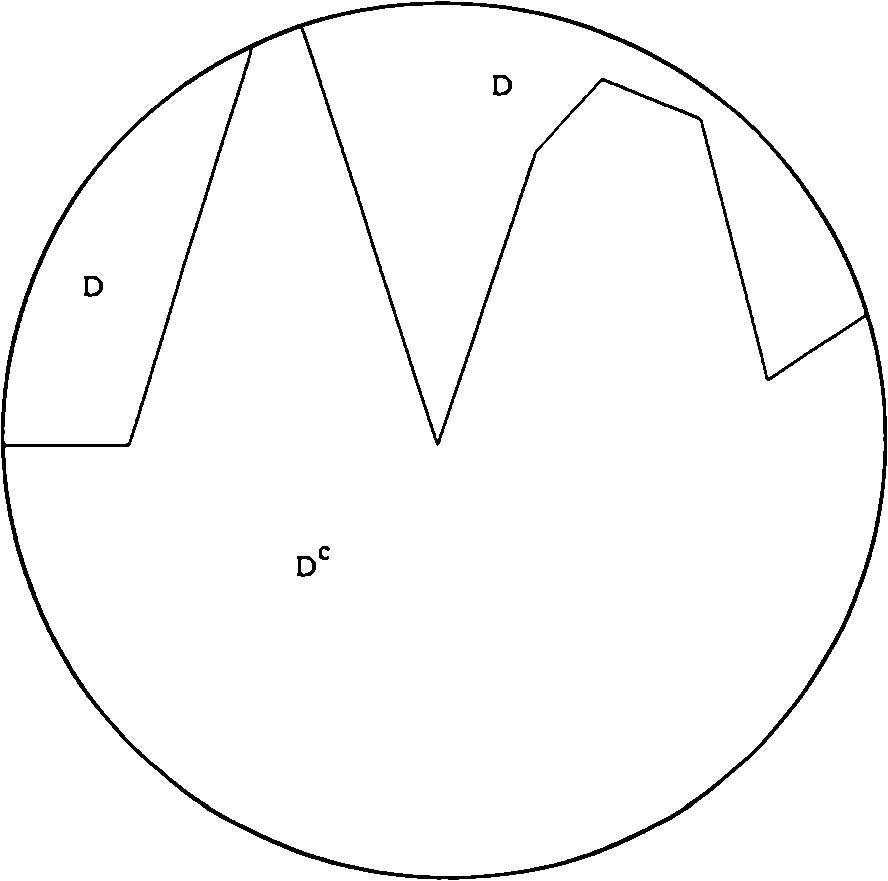
\includegraphics{Images/Img5.png}
    \caption{A Lipschitz domain such that $D\cap B(x,r)$ has more than one com\-ponent.}
    \label{fig:ch3_1.1}
\end{figure}

Let us make the observation that if $D$ is the region above the graph of a Lipschitz function $\Gamma$ and $a > 0$, then $aD = \{ay : y \in D\}$ is the region above the function $\Gamma_a$, where $\Gamma_a(x) = a\Gamma(x/a)$. Note
\[
    |\Gamma_a(z_1) - \Gamma_a(z_2)| = a|\Gamma(z_1/a) - \Gamma(z_2/a)| \leq aM_\Gamma|z_1/a - z_2/a|,
\]
and so $\Gamma_a$ has the same Lipschitz constant as $\Gamma$. We will call this property ``scaling.''\index{Scaling}

\index{Lipschitz domain|)}

We can now give a precise statement of the boundary Harnack principle for Lipschitz domains.

\begin{theorem}\label{thm:ch3_1.2}
Suppose $D$ is a connected Lipschitz domain, $x_0 \in D$. Suppose $V$ is open, $K$ is compact, and $K \subseteq V$. Then there exists a constant $c$, depending only on $K$, $V$, and $D$, such that if $u$ and $v$ are two positive harmonic functions on $D$ that both vanish continuously on $V \cap \partial D$, then
\begin{equation}\label{eq:ch3_1.3}
    u(x)/v(x) \leq cu(x_0)/v(x_0), \qquad x \in K \cap D.
\end{equation}
\end{theorem}

Saying that a harmonic function $u$ vanishes continuously on $V \cap \partial D$ means that $u(x)$ tends to $0$ as $x$ tends to $z$ uniformly over $z$ in compact subsets of $V \cap \partial D$.

Reversing the roles of $u$ and $v$, $v(y)/u(y) \leq c_1v(x_0)/u(x_0)$ for $y \in K \cap D$. Combining, we obtain the following corollary of Theorem \ref{thm:ch3_1.2}.

\begin{corollary}\label{cor:ch3_1.3}
Suppose $K,V$, and $D$ are as in Theorem \ref{thm:ch3_1.2}. There exists $c$ such that if $u$, $v$ are positive harmonic on $D$ with $u$, $v$ vanishing continuously on $V \cap \partial D$, then
\begin{equation}\label{eq:ch3_1.4}
u(x)/v(x) \leq cu(y)/v(y), \qquad x,y \in K \cap D.
\end{equation}
\end{corollary}

The function $u/v$ is ``harmonic'' with respect to the probability measures $\P_v^x$ (see \chapeqref[I]{eq:ch1_6.16} for the definition of $\P_v^x$). That is, if $S$ is a stopping time less than $\tau_D$, then since $u$ is harmonic,
\[
    \E_v^x\Big(\frac{u}{v}\Big)(X_{t\wedge S}) = \E^x\Big(\frac{u}{v}\Big)(X_{t\wedge S})\frac{v(X_{t\wedge S})}{v(x)} = \E^xu(X_{t\wedge S})/v(x) = u(x)/v(x).
\]
One way to think of the boundary Harnack principle\index{Boundary Harnack principle}, then, is as the ordinary Harnack inequality for positive functions that are $L_v$-harmonic, i.e., $L_vu = 0$, where $L_v$ is the operator corresponding to Brownian motion conditioned by the function $v$. This means that
\begin{equation}\label{eq:ch3_1.5}
    L_vu = \frac{1}{2}\Delta u + \frac{\nabla v}{v} \cdot \nabla u.
\end{equation}

\subsecbkm{ch3_sec1.2}{The box method}
\index{Box method|(}

It will turn out that to prove the boundary Harnack principle, the key situation to consider is the case of a domain above the graph of a Lipschitz function. For now suppose $\Gamma$ is a bounded Lipschitz function on $\R^{d-1}$ and
\mpagebreak
\[
    D = \{x : x^d > \Gamma(x^1,\ldots,x^{d-1})\}.
\]
Define the vertical distance from $x$ to $\partial D$ by
\begin{equation}\label{eq:ch3_1.6}
    \delta(x) = x^d - \Gamma(x^1,\ldots,x^{d-1}).
\end{equation}
Note that since this is a Lipschitz domain, there exists a constant $c$ depending only on $M_\Gamma$ such that
\begin{equation}\label{eq:ch3_1.7}
    c\delta(x) \leq \dist(x,\partial D) \leq \delta(x).
\end{equation}
Define the ``box''
\begin{align}\label{eq:ch3_1.8}
    Q(x,a,R) &= \{y \in D : \delta(y) < a, \\
    &\qquad\,\,|(y^1,\ldots,y^{d-1})-(x^1,\ldots,x^{d-1})| < R\}. \notag
\end{align}
We will let $U$ be the upper boundary of $Q$:
\begin{equation}\label{eq:ch3_1.9}
    U(x,a,R) = \{y \in \partial Q(x,a,R) : \delta(y) = a\},
\end{equation}
and $S$ the sides:
\begin{align}\label{eq:ch3_1.10}
    S(x,a,R) &= \{y \in \partial Q(x,a,R) : \\
    &\qquad\,\,|(y^1,\ldots,y^{d-1})-(x^1,\ldots,x^{d-1})| = R\}. \notag
\end{align}
For any two points $x$ and $y$ we say that $y$ is ``above'' $x$ or $x$ is ``below'' $y$ if $(y^1,\ldots,y^{d-1}) = (x^1,\ldots,x^{d-1})$ and $y^d \geq x^d$.

As we will see (Theorem \ref{thm:ch3_1.7}), what we need to show is that the probability of exiting $Q(x,a,R)$ through the sides is less than a constant times the probability of exiting through the top, provided we do not start too near the sides. The point is that the process does not exit $Q(x,a,R)$ by creeping along the boundary.

Since $D$ is the region above a Lipschitz function, clearly it satisfies the exterior cone condition, and hence every point of $\partial D$ is regular for $D^c$ (see Proposition \chapref[II]{prop:ch2_1.13}). We want to make a stronger uniform statement.

\begin{lemma}\label{lem:ch3_1.4}
There exists $\rho < 1$ such that if $z \in D$ and $a = \delta(z)$, then
\[
   \frac{|\partial B(z,2a) \cap D|}{|\partial B(z,2a)|} \leq \rho.
\]
\end{lemma}

\begin{proof}
By a scaling argument, we may assume $a = 1$. Without loss of generality, make a change of coordinates so that $z = (0,\ldots,0,1)$. By the definition of $\delta(z)$, the point $0 \in \partial D$. Since $\Gamma$ is Lipschitz, there exists $c_1$ such that the set $A = \{x \in \partial B(z,2) : |x-(0,\ldots,0,-1)| \leq 1/c_1\} \subseteq D^c$. Note there exists $c_2$ such that $|A| \geq c_2|\partial B(z,2)|$. The result now follows by taking $\rho = 1-c_2$.
\end{proof}

Since the distribution of $X_{\tau(B(z,2a))}$, started at $z$, is uniform on the boundary of $\partial B(z,2a)$, we conclude
\begin{equation}\label{eq:ch3_1.11}
    \P^z(X_{\tau(B(z,2a))} \in D) \leq \rho.
\end{equation}
We use this to find an upper bound on the probability of exiting $Q(x,a,R)$ through the sides.

\begin{lemma}\label{lem:ch3_1.5}
There exist $c_1$ and $c_2$ such that if $y \in Q(x,a,R/2)$, then
\[
    \P^y(X_{\tau(Q(x,a,R))} \in S(x,a,R)) \leq c_1\exp(-c_2R/a).
\]
\end{lemma}

\begin{proof}
Suppose first that $R > 24a$. Let
\[
    V_1 = \inf\{t > 0 : |X_t-X_0| \geq 2a\}, \qquad V_{i+1} = V_i + V_1 \circ \theta_{V_i}, \qquad i = 1,2,\ldots.
\]
The $V_i$ are the successive times that the process $X_t$ moves $2a$ (cf.\ Sect.\ \chapref[I]{ch1_sec3}).

Let us write $\tau_Q$ for $\tau_{Q(x,a,R)}$. Note that $|X_{V_i} - X_0| \leq 2ai$. Thus, if $X_{\tau_Q} \in S(x,a,R)$, we must have $\tau_Q > V_{\lfloor R/8a \rfloor}$, $\P^y$-a.s.\ if $y \in Q(x,a,R/2)$. By the strong Markov property,
\begin{align*}
    \P^y(\tau_Q > V_{i+1}) &\leq \P^y(\tau_Q > V_i, \tau_Q \circ \theta_{V_i} > V_1 \circ \theta_{V_i}) \\
    &= \E^y\big[\P^{X_{V_i}}(\tau_Q > V_1); \tau_Q > V_i\big].
\end{align*}

If $i \leq R/8a$ and $\tau_Q > V_i$, then $|X_{V_i} - X_0| \leq R/4$ and $X_{V_i} \in Q(x,a,3R/4)$, $\P^y$-a.s. Hence $\P^{X_{V_i}}(\tau_Q > V_1) \leq \rho$ by Lemma \ref{lem:ch3_1.4}. So
\[
    \P^y(\tau_Q > V_{i+1}) \leq \rho\P^y(\tau_Q > V_i).
\]
By induction,
\begin{align*}
    \P^y(X_{\tau_Q} \in S(x,a,R)) &\leq \P^y(\tau_Q > V_{\lfloor R/8a \rfloor}) \leq \rho^{\lfloor R/8a \rfloor} \\
    &= \exp(\lfloor R/8a \rfloor \log \rho) \leq c_1\exp(-c_2R/a).
\end{align*}
(Since $\rho < 1$, $\log \rho < 0$.) This gives our result when $R > 24a$. We have the result for $R \leq 24a$ by taking $c_1$ large enough.
\end{proof}

Not surprisingly, we now want a lower bound on leaving $Q(x,a,R)$ through the top.

\begin{lemma}\label{lem:ch3_1.6}
There exist $c$ and $\beta > 0$ such that if $a \leq 1/2$, $y \in Q(x,a,a/2)$, and $b = \delta(y) \leq a$, then
\[
    \P^y(X_{\tau(Q(x,1,4))} \in U(x,1,4)) \geq cb^\beta.
\]
\end{lemma}

\begin{proof}
Let $y_0 = y = (y^1,\ldots,y^{d-1},y^d)$. We will construct a sequence of points $y_i = (y^1,\ldots,y^{d-1},y_i^d)$ above $y$ for $i=1,\ldots,n$ for some $n$ by choosing $y_i^d$ so that
\mpagebreak
\[
    |y_i - y_{i-1}| = r_i = \dist(y_{i-1},\partial D)/4
\]
and $\delta(y_n) \geq 2$. Once we have this sequence, we let $B_i = B(y_i,2r_i)$ and $B = \cup_{i=0}^n B_i$. By our construction $B \subseteq Q(x,4,4)$. We define
\[
    h(z) = \P^z(X_{\tau_B} \in \partial B - Q(x,1,4)).
\]
So $h$ is the harmonic function on $B$ with boundary value $1$ on $\partial B-Q(x,1,4)$ and $0$ on the rest of $\partial B$.

By the support theorem (Theorem \chapref[I]{thm:ch1_6.6}), there exists $c_1$ such that
\[
    \P^0(\sup_{s\leq 2}|X_s - \psi(s)| < 1/8) \geq c_1,
\]
where $\psi(s)$, $0 \leq s \leq 2$, is the curve that moves upward at constant unit speed: $\psi(s) = (0,\ldots,0,s)$. If $A = \{x \in \partial B(0,1) : x^d > 0, |(x^1,\ldots,x^{d-1}| < 1/8\}$ then $\P^0(X_{\tau(B(0,1))} \in A) \geq c_1$. By translation invariance and scaling,
\[
    \P^{y_n}(X_{\tau(B(y_n,r_n))} \in Q(x,1,4)) \geq c_1.
\]
and therefore $h(y_n) \geq c_1$. By the usual Harnack inequality (Theorem \chapref[II]{thm:ch2_1.19}), there exists $c_2$ such that $h(y_i) \geq c_2h(y_{i+1})$ for each $i$. By induction, $h(y_0) \geq c_1c_2^n = c_1\exp(n\log c_2)$. Since $c_2 < 1$, this is equal to $c_1\exp(-c_3n)$ for some $c_3 > 0$. If $X_t$ exits $B$ through $\partial B - Q(x,1,4)$, then $X_t$ exits $Q(x,1,4)$ through $U(x,1,4)$. Hence $\P^y(X_{\tau(Q(x,1,4))} \in U(x,1,4)) \geq \P^y(X_{\tau_B} \in \partial B - Q(x,1,4))$, and we will have our result once we figure out what $n$ must be.

Now $r_i \geq \dist(y_{i-1},\partial D)/4$ and by our construction, is increasing in $i$. So $r_1 \geq \delta(y_0)/4M_\Gamma \geq b/4M_\Gamma$. Let $m = [8M_\Gamma] + 1$. Then $\delta(y_m) \geq mr_1 \geq 2b$. So $r_m \geq b/2M_\Gamma$. Repeating, we see that $\delta(y_{2m}) \geq mr_m \geq 4b$, and by induction, $\delta(y_{km}) \geq 2^k b$. We choose $n$ to be $km$ where $k$ is the first integer such that $2^k b > 2$. So $k = [\log(2/b)/\log 2] + 1 \leq -c_4\log b$. Hence $n \leq -c_5\log b$, or
\[
    c_1\exp(-c_3n) \geq c_1\exp(c_3c_5\log b) = c_1b^\beta
\]
with $\beta = c_3c_4$.
\end{proof}

We finally can make precise the notion that the probability that the process leaves $Q(x,a,R)$ through the sides is not too high. We suppose $a \leq 1/2$, $R \geq 8a$. Define
\begin{align}\label{eq:ch3_1.12}
    H_1 &= (X_{\tau(Q(x,a,R))} \in S(x,a,R)), \\
    H_2 &= (X_{\tau(Q(x,a,R))} \in U(x,a,R)). \notag
\end{align}

\begin{theorem}\label{thm:ch3_1.7}
There exists $c$ such that if $y \in Q(x,a,R/2)$, then $\P^y(H_1) \leq c\P^y(H_2)$.
\end{theorem}

\begin{proof}
By a scaling argument, it suffices to show our result for the case $a = 1/2$. Since increasing $R$ increases $\P^y(H_2)$ but decreases $\P^y(H_1)$, it is enough to prove our result when $R = 4$. Let
\begin{equation}\label{eq:ch3_1.13}
    r_i = R\bigg(\frac{3}{4} - \frac{1}{40}\sum_{j=1}^i \frac{1}{j^2}\bigg).
\end{equation}
Note $R/2 \leq r_1 \leq R$ for all $i$. (Recall that $\sum_{j=1}^\infty j^{-2} = \pi^2/6 \approx 1.5$; see any book on Fourier series, e.g., \cite{Folland1992}, for a proof.) Let
\[
    J_i = Q(x,2^{-i},r_i) - Q(x,2^{-i-1},r_i)
\]
and let
\[
    d_i = \sup_{y\in J_i} \P^y(H_1)/\P^y(H_2).
\]

\bigskip
\begin{figure}[ht]
    \centering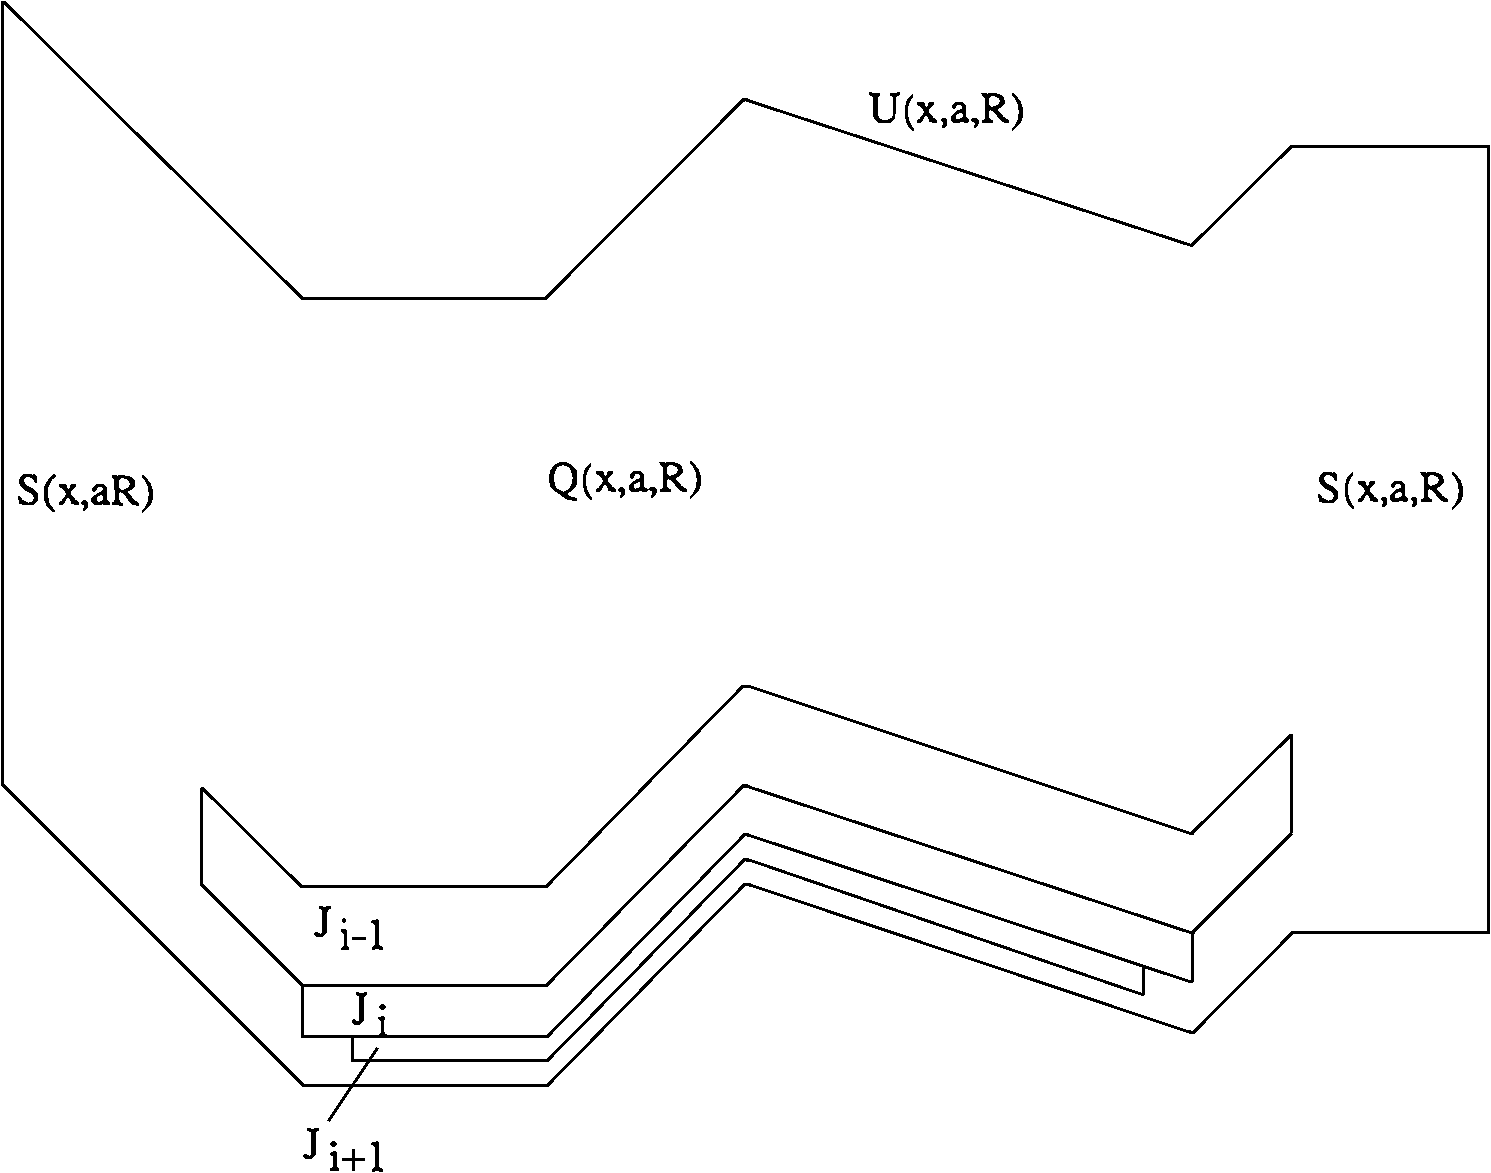
\includegraphics{Images/Img6.png}
    \bigskip
    \caption{The sets $J_i$.}
    \label{fig:ch3_1.2}
\end{figure}

For $y \in Q(x,a,R/2)-\cup_{i=2}^\infty J_i$, we have by Lemma \ref{lem:ch3_1.6} that $\P^y(H_2) \geq c$. So
\[
    \P^y(H_1)/\P^y(H_2) \leq 1/c < \infty
\]
for $y$ in this set, or $d_1 \leq 1/c < \infty$.

\mpagebreak

Our aim is to bound $d_i$ in terms of $d_{i-1}$. Suppose $y \in J_i$, write $\tau_i$ for $\tau_{Q(x,2^{-i},r_{i-1})}$, and write $\tau_Q$ for $\tau_{Q(x,a,R)}$. If $X_t$ started at $y$ exits $Q(x,a,R)$ through its sides $S(x,a,R)$, either it exits $Q(x,2^{-i},r_{i-1})$ through $S(x,2^{-i},r_{i-1})$ or it exits $Q(x,2^{-i},r_{i-1})$ through the top $U(x,2^{-i},r_{i-1})$ and then exits $Q(x,a,R)$ through $S(x,a,R)$. So we have
\begin{align}\label{eq:ch3_1.14}
    \P^y(H_1) &\leq \P^y\big(X_{\tau_i} \in S(x,2^{-i},r_{i-1})\big) \\
    &\qquad+ \P^y\big(X_{\tau_i} \in U(x,2^{-i},r_{i-1}); X_{\tau_Q} \in S(x,a,R)\big). \notag
\end{align}
By Lemma \ref{lem:ch3_1.5} and some algebra, the first term on the right-hand side of \eqref{eq:ch3_1.14} is less than or equal to
\begin{equation}\label{eq:ch3_1.15}
    c_1e^{-c_2(r_{i-1}-r_i)/2^{-i}} \leq c_1e^{-c_22^i/i^2} \leq c(2^{-i})^\beta/i^2.
\end{equation}
Here we used \eqref{eq:ch3_1.13}. Since $X_{\tau_Q} = X_{\tau_Q} \circ \theta_{\tau_i}$, the strong Markov property at time $\tau_i$ bounds the second term on the right in \eqref{eq:ch3_1.14} by
\begin{equation}\label{eq:ch3_1.16}
    \E^y\big[\P^{X_{\tau_i}}(H_1); X_{\tau_i} \in U(x,2^{-i},r_{i-1})\big].
\end{equation}
Since $X_{\tau_i} \in U(x,2^{-i},r_{i-1})$ implies $X_{\tau_i} \in J_{i-1}$, \eqref{eq:ch3_1.16} in turn is bounded by
\begin{align}\label{eq:ch3_1.17}
    d_{i-1}\E^y\big[\P^{X_{\tau_i}}(H_2)&; X_{\tau_i} \in U(x,2^{-i},r_{i-1})\big] \\
    &\leq d_{i-1}\P^y(X_{\tau_Q} \in U(x,a,R)) \notag \\
    &\leq d_{i-1}\P^y(H_2). \notag&
\end{align}
Combining \eqref{eq:ch3_1.14}, \eqref{eq:ch3_1.15}, and \eqref{eq:ch3_1.17},
\[
    \P^y(H_1)\le c2^{-i\beta}/i^2 + d_{i-1}\P^y(H_2).
\]

By Lemma \ref{lem:ch3_1.6}, for $y \in J_i$,
\[
    \P^y(H_2) \geq c(2^{-i})^\beta.
\]
Hence
\[
    \P^y(H_1)/\P^y(H_2) \leq (c/i^2)\P^y(H_2) + d_{i-1}\P^y(H_2).
\]
Taking the supremum over $y$s in $J_i$,
\[
    d_i \leq d_{i-1} + c/i^2.
\]
Therefore
\[
    d_i \leq d_1 + c\sum_{j=1}^i \frac{1}{j^2}
\]
or $\sup_i d_i < \infty$. This is exactly what we needed to prove.
\end{proof}

The other key step is the following proposition, known as a Carleson estimate\index{Carleson estimate|(}.

\mpagebreak

\begin{theorem}\label{thm:ch3_1.8}
Suppose $u$ is positive and harmonic in $D$, the region above the graph of a Lipschitz function $\Gamma$. Let $x \in D$, suppose $u(x) = 1$, and suppose $u$ vanishes continuously on $B(x,4\delta(x)) \cap \partial D$. There exists $c$, not depending on $x$ or $u$, such that $u(y) \leq c$ for all $y \in D \cap B(x,2\delta(x))$.
\end{theorem}

\begin{proof}
By a scaling argument, we may suppose $\delta(x) = 1$. By the usual Harnack inequality, $u \leq c$ on $U(x,1,4)$. If $y_1 \in U(x,1,4)$ and $y$ lies directly below $y_1$, then by Exercise \ref{ex:ch3_4} we see that there exists $\beta$ such that
\begin{equation}\label{eq:ch3_1.18}
    u(y) \leq c_1\delta(y)^{-\beta}.
\end{equation}
So if $u(y) \geq M$, then $\delta(y) \leq (c_1/M)^{1/\beta}$.

Take $N$ large. Suppose there exists $x_1 \in B(x,2) \cap D$ with $u(x_1) \geq N$. We will construct a sequence $x_i$ tending to a point in $B(x,4) \cap \partial D$ with $u(x_i) \to \infty$, which is a contradiction. Let $r_1 = \dist(x_1,\partial D)$. Using \eqref{eq:ch3_1.11}, there exists $\rho < 1$ not depending on $x_1$ such that
\begin{align*}
    N &\leq u(x_1) = \E^{x_1}u(X_{\tau(B(x_1,2r_1))}) \\
    &= \E^{x_1}[u(X_{\tau(B(x_1,2r_1))}); \tau_{B(x_1,2r_1)} < \tau_D] \\
    &\leq \rho \sup_{\partial B(x_1,2r_1)} u.
\end{align*}

Therefore there must exist $x_2$ in $\partial B(x_1,2r_1) \cap D$ with $u(x_2) \geq N/\rho$. Keep repeating the above argument, with $x_1$ and $r_1$ replaced by $x_i$ and $r_i = \dist(x_i,D)$. As long as $B(x_i,2r_i) \subseteq B(x,3)$, there will exist $x_{i+1} \in \partial B(x_i,2r_i) \cap D$ with $u(x_{i+1}) \geq u(x_i)/\rho$. This implies $u(x_i) \geq N/\rho^{i-1}$. In turn, by \eqref{eq:ch3_1.7} and \eqref{eq:ch3_1.18},
\[
    r_i \leq \delta(x_i) \leq cu(x_i)^{-1/\beta} \leq c\frac{(\rho^{i-1})^{1/\beta}}{N^{1/\beta}}.
\]
The sum $\sum r_i$ converges, and if we take $N$ large enough, the sum will be less than $1/4$. Since $x_{i+1} \in \partial B(x_i,2r_i) \cap D$, $|x_{i+1} - x_i| = 2r_i$ and
\[
    |x_i - x| \leq |x_i - x_1| + |x_1 - x| \leq \sum_{j=1}^i 2r_j + 2 < 5/2,
\]
hence $B(x_i,2r_i) \subseteq B(x,3)$. With this choice of $N$, we thus obtain a sequence $x_1,x_2,\ldots$ such that $\dist(x_i,\partial D) \to 0$, $u(x_i) \to \infty$, and $B(x_i,2r_i) \subseteq B(x,3)$. Since every point on the boundary of $D$ is regular for $D^c$, this contradicts the fact that $u = 0$ on $B(x,4) \cap \partial D$. Therefore we conclude that $u$ is bounded on $B(x,2) \cap D$ by $N$.
\end{proof}

\index{Carleson estimate|)}

Finally we can put Theorems \ref{thm:ch3_1.7} and \ref{thm:ch3_1.8} together to prove Theorem \ref{thm:ch3_1.2}.

\begin{proof}[Proof of Theorem \ref{thm:ch3_1.2}]
For the moment, let us continue to suppose that $D$ is the region above the graph of a bounded Lipschitz function. Suppose $\delta(x_0) \in [2,4]$. Write just $Q$ for $Q(x_0,1/2,4)$ and similarly $U$, $S$. Then, by the usual Harnack inequality, $\sup_U u \leq cu(x_0)$ and $\inf_U v \geq cv(x_0)$. If $x \in Q(x_0,1/2,2)$, we write
\begin{align}\label{eq:ch3_1.19}
    u(x) &= \E^x[u(X_{\tau_Q}); X_{\tau_Q} \in S] + \E^x[u(X_{\tau_Q}); X_{\tau_Q} \in U] \\
    &\leq c(\sup_U u)\P^x(X_{\tau_Q} \in S) + cu(x_0)\P^x(X_{\tau_Q} \in U) \notag \\
    &\leq cu(x_0)\P^x(X_{\tau_Q} \in S) + cu(x_0)\P^x(X_{\tau_Q} \in U) \notag
\end{align}
by Theorem \ref{thm:ch3_1.8}. Using Theorem \ref{thm:ch3_1.7}, this is less than or equal to
\begin{align*}
    cu(x_0)\P^x(X_{\tau_Q} \in U) &\leq c\frac{u(x_0)}{v(x_0)}\E^x[v(X_{\tau_Q}); X_{\tau_Q} \in U] \\
    &\leq c\frac{u(x_0)}{v(x_0)}v(x).
\end{align*}

This gives our result in this special case. By scaling, we have the boundary Harnack principle for domains above the graph of a Lipschitz function, without assuming anything on $\delta(x_0)$.

Finally, cover $K$ by a finite number of balls contained in $V$ whose radii are small enough that the intersection of $D$ with any one of these balls is the same as the intersection of the region above the graph of some Lipschitz function with the same ball (recall the definition of a Lipschitz domain). For each small ball $B_i$, take a point $x_i$. We have shown that $u(y)/v(y) \leq cu(x_i)/v(x_i)$ for all $y \in B_i$. By the usual Harnack inequality, $u(x_i) \leq cu(x_0)$ and $v(x_i) \geq cv(x_0)$, so $u(x_i)/v(x_i) \leq c^2u(x_0)/v(x_0)$. Putting this all together and remembering there are only finitely many $B_i$, we deduce $u(y)/v(y) \leq cu(x_0)/v(x_0)$, which is what we wanted to prove.
\end{proof}

\index{Box method|)}

\tweakpage{0.6}

\subsecbkm{ch3_sec1.3}{The SDE method}
\index{S2@SDE method|(}

We now proceed to give another proof of the boundary Harnack principle in Lipschitz domains, the ``SDE'' method. SDE is an abbreviation for ``stochastic differential equations'' (cf.\ Sect.\ \chapref[I]{ch1_sec6}). Although this method gives the boundary Harnack principle for many of the same domains for which the box method works (see the Extensions subsection), the box method seems to be the more versatile of the two. Nevertheless, the SDE method is more useful for proving Harnack inequalities for operators similar to ones like $L_v$ in \eqref{eq:ch3_1.5} but that are not given by an $h$-path transform. As part of our discussion of the SDE method, we will obtain some estimates on harmonic functions that are of considerable interest in themselves.

\begin{lemma}\label{lem:ch3_1.9}
Suppose $D$ is the region above the graph of a Lipschitz function $\Gamma$ and $x_1 \in D$. There exist $c_1,c_2$ and $\beta_1,\beta_2 > 0$ such that if $u$ is positive and harmonic in $D$ and $u(x_1) = 1$, then for $x$ below $x_1$,
\mpagebreak
\begin{equation}\label{eq:ch3_1.20}
    u(x) \leq c_1\delta(x)^{-\beta_1}
\end{equation}
and
\begin{equation}\label{eq:ch3_1.21}
    u(x) \geq c_2\delta(x)^{\beta_2}.
\end{equation}
In addition, if $u$ vanishes continuously on $B(x_1,4\delta(x_1)) \cap \partial D$, then there exists $c_3$ and $\beta_3 > 0$ such that
\begin{equation}\label{eq:ch3_1.22}
    u(x) \leq c_3\delta(x)^{\beta_3}.
\end{equation}
\end{lemma}

\begin{proof}
The first and second inequalities were essentially proved in Lemma \ref{lem:ch3_1.6}; see Exercise \ref{ex:ch3_4}. The third inequality we deduce from the Carleson estimate as follows. Without loss of generality, we may assume $\delta(x_1) = 1$ (scaling). By the usual Harnack inequality and Carleson's estimate, there exists $K$ such that $u(y) \leq K$ for all $y \in Q(x_1,1,2)$. Let $M = 4M_\Gamma \vee 16$. Now suppose $z \in Q(x_1,M^{-1},3/2)$. By \eqref{eq:ch3_1.11} there exist $\rho < 1$ so that
\begin{align*}
    u(z) &= \E^z u(X_{\tau(B(z,2M^{-1}))\wedge\tau_D}) \\
    &\leq \big(\sup_{Q(x_1,1,2)} u\big)\P^z(X_{\tau_{B(z,2M^{-1})}\wedge \tau_D} \in D) \\
    &\leq \rho K.
\end{align*}
Repeat: if $z \in Q(x_1,M^{-2},5/4)$,
\begin{align*}
    u(z) &= \E^z u(X_{\tau(B(z,2M^{-2}))\wedge\tau_D}) \\
    &\leq \big(\sup_{Q(x_1,M^{-1},3/2)} u\big)\P^z(X_{\tau_{B(z,2M^{-2})}\wedge \tau_D} \in D) \\
    &\leq \rho(\rho K).
    % Note: removed extra parentheses in line 2
\end{align*}
Continuing, if $z \in Q(x_1,M^{-n},1+(1/2)^n)$, then $u(z) \leq K\rho^n$. \eqref{eq:ch3_1.22} follows from this with some algebra.
\end{proof}

Let $h$ be the positive harmonic function in $Q(x,a,R)$ that has boundary value $1$ on $S(x,a,R)$ and $U(x,a,R)$ and boundary value $0$ on $\partial D \cap \partial Q(x,a,R)$. The reason we look at this particular harmonic function is that
\begin{align}\label{eq:ch3_1.23}
    \P_h^y\big(X_{\tau(Q(x,a,R))} &\in S(x,a,R)\big) \\
    &= \P^y\big(X_{\tau(Q(x,a,R))} \in S(x,a,R)\big)/h(y) \notag
\end{align}
since $h$ is $1$ on $S(x,a,R)$, with a similar equation for $U(x,a,R)$. So if we prove
\begin{equation}\label{eq:ch3_1.24}
    \P_h^y\big(X_{\tau(Q(x,a,R))} \in S(x,a,R)\big) \leq c\P_h^y\big(X_{\tau(Q(x,a,R))} \in U(x,a,R)\big),
\end{equation}
we can then multiply by $h(y)$ to obtain the conclusion of Theorem \ref{thm:ch3_1.7}. From then on the proof via the SDE method proceeds the same as the proof via the box method.

For this $h$ we have the following.

\begin{lemma}\label{lem:ch3_1.10}
There exist $c$ such that if $y \in Q(x,a/2,R/2)$, then
\[
    \frac{|\nabla h(y)|}{h(y)} \geq \frac{c}{\delta(y)}.
\]
\end{lemma}

Note that this inequality is sharp, since by Corollary \chapref[II]{cor:ch2_1.4} and Harnack's inequality,
\[
    |\nabla h(y)| \leq \frac{c}{\dist(y,\partial D)}\Big(\sup_{B(y,\dist(y,\partial D)/2)} h\Big) \leq \frac{c}{\delta(y)}h(y).
\]

\begin{proof}
Fix $y$. If $y_1$ is directly below $y$, then by Lemma \ref{lem:ch3_1.9} and scaling, there exists $\beta$ such that
\[
    h(y_1) \leq c_1h(y)[\delta(y_1)/\delta(y)]^\beta.
\]
Choose $y_1$ below $y$ so that
\[
    \delta(y_1) = (2c_1)^{-1/\beta}\delta(y).
\]
Hence $h(y_1) \leq h(y)/2$. By the mean value theorem, there exists $y_2$ between $y_1$ and $y$ such that
\[
    \frac{1}{2}h(y) \leq h(y) - h(y_1) = \frac{\partial h}{\partial x^d}(y_2)|\delta(y) - \delta(y_1)|,
\]
or
\[
    \frac{\partial h}{\partial x^d}(y_2) \geq \frac{ch(y)}{\delta(y)}.
\]

Now consider $\partial h/\partial x^d$. We want to show it is nonnegative. Since $h = 1$ on $S(x,a,R)$, then $\partial h/\partial x^d = 0$ on $S(x,a,R)$. Since $h = 0$ on $\partial D$ and $h \geq 0$ in $D$, then $\partial h/\partial x^d \geq 0$ on $\partial D \cap \overline{Q(x,a,R)}$. Since $h = 1$ on $U(x,a,R)$ and $h \leq 1$ in $Q(x,a,R)$, then $\partial h/\partial x^d \geq 0$ on $U(x,a,R)$. Therefore the boundary values of $\partial h/\partial x^d$ are nonnegative, and hence $\partial h/\partial x^d$ is a nonnegative harmonic function in $Q(x,a,R)$.

Since $\dist(y_2,\partial D) \geq c\delta(y_2) \geq c\delta(y_1) \geq c\delta(y)$ and $|y_2 - y_1| \leq c\delta(y)$, it follows by the Harnack inequality that
\[
    \frac{\partial h}{\partial x^d}(y) \geq c\frac{\partial h}{\partial x^d}(y_2) \geq c\frac{h(y)}{\delta(y)}.
\]
Since $|\nabla h(y)| \geq (\partial h/\partial x^d)(y)$, our result follows.
\end{proof}

We have seen in \chapeqref[I]{eq:ch1_6.19} that under $\P_h^x$, $X_t$ satisfies the stochastic differential equation
\mpagebreak
\begin{equation}\label{eq:ch3_1.25}
    dX_t = dW_t + (\nabla h/h)(X_t)dt,
\end{equation}
where $W_t$ is a $d$-dimensional Brownian motion. So an easy calculation using It\^o's lemma tells us that if $\alpha \in (0,1)$ and $Y_t = h^\alpha(X_t)$, then
\begin{align}\label{eq:ch3_1.26}
    dY_t &= \alpha h^{\alpha-1}(X_t)\nabla h(X_t) \cdot dW_t \\
    &\qquad+ (\alpha(\alpha+1)/2)h^{\alpha-2}(X_t)|\nabla h(X_t)|^2 dt, \qquad t < \tau_D, \notag
\end{align}
using the fact that $\Delta h \equiv 0$. We let $M_t$ denote the martingale part of $Y_t$, that is,
\[
    M_t = \int_0^{t\wedge\tau_D} \alpha h^{\alpha-1}(X_t)\nabla h(X_t) \cdot dW_t,
\]
and we let $B_t$ denote the bounded variation part of $Y_t$, that is,
\[
    B_t = \int_0^{t\wedge\tau_D} (\alpha(\alpha+1)/2)h^{\alpha-2}(X_t)|\nabla h(X_t)|^2 dt.
\]
Let
\[
    A_t = \int_0^t \frac{|\nabla h|}{h}(X_s)ds.
\]

The idea of the SDE proof is as follows. In a short time $t_0$, a Brownian motion will not travel far. So in order for $X_t$ to go a large distance in time $t_0$, $A_{t_0}$ must be large. Either $h(X_t)$ also becomes large in that time, or else by comparing $B_t$ to $A_t$, we see that $B_{t_0}$ is large. If $B_{t_0}$ is large, then provided we can control the martingale term in \eqref{eq:ch3_1.26}, $Y_t = h^\alpha(X_t)$ must become large. In either case, $h(X_t)$ is not too small, which says that $X_t$ does not stay too close to the boundary.

% Note changed "Proof of Theorem 1.1" to "Proof of Theorem 1.2"

\begin{proof}[Proof of Theorem \ref{thm:ch3_1.2}, SDE method]
Let $X_t$ be the solution to \eqref{eq:ch3_1.25}. Let $s$ be a number to be chosen in a moment and let
\begin{align*}
    S = \inf\{t : |X_t - x_0| \geq &1/2\}, \qquad \sigma_s = \inf\{t : h(X_t) > s\}, \\
    &\rho = \inf\{t : B_t \geq 1\}.
\end{align*}
Let $b = \beta_2$ be the exponent from Lemma \ref{lem:ch3_1.9} and set $\alpha = 1/2b$. First we compare $\lrang{M}_t$ and $A_t$ to $B_t$. Note
\begin{equation}\label{eq:ch3_1.27}
    \frac{|\nabla h|}{h}(x) \geq \frac{c}{\delta(x)} \geq \frac{c}{h(x)^{1/b}}
\end{equation}
from Lemma \ref{lem:ch3_1.10}, and so
\begin{equation}\label{eq:ch3_1.28}
    \frac{|\nabla h|}{h}\frac{|\nabla h|}{h}h^\alpha \geq \frac{|\nabla h|}{h}\frac{1}{h^\alpha}.
\end{equation}
Hence
\begin{equation}\label{eq:ch3_1.29}
    B_{t\wedge\sigma_s} \geq Ks^{-\alpha}A_{t\wedge\sigma_s}
\end{equation}
\mnewpage
for some $K > 0$. Also,
\begin{equation}\label{eq:ch3_1.30}
    \lrang{M}   _{t\wedge\sigma_s} = \int_0^{t\wedge\sigma_s} \alpha^2h^{2\alpha-2}(X_t)|\nabla h(X_t)|^2 dt \leq c_2s^\alpha B_{t\wedge\sigma_s}.
\end{equation}

Next we partition our probability space into five sets $D_1,\ldots,D_5$. Let
\[
    D_1 = (\sigma_s \leq S), \qquad D_2 = (\sup_{u\leq t_0} |W_u| \geq 1/4),
\]
where $t_0$ is also a number to be chosen in a moment. If $\omega$ is not in $D_1 \cup D_2$, then $\sigma_s > S$ and either $S \leq t_0 \wedge \rho$ or $S > t_0 \wedge \rho$. If $S > t_0 \wedge \rho$, either $t_0 < \rho$ or $t_0 \geq \rho$. Hence if we let
\[
    D_3 = (\sigma_s > S, S \leq t_0 \wedge \rho) \cap D_2^c, \qquad D_4 = (\sigma_s > S > t_0, \rho > t_0),
\]
and
\[
    D_5 = (\sigma_s > S > \rho, t_0 \geq \rho),
\]
then $\Omega = D_1 \cup D_2 \cup D_3 \cup D_4 \cup D_5$.

Now we show that the probabilities of $D_2$ and $D_5$ are small, while $D_3$ and $D_4$ must be empty. Choose $t_0$ small so that $2\exp(-1/32t_0) < 1/4$. Hence $\P_h^x(D_2) < 1/4$. Choose $s < 4^{-1/\alpha}$ small so that $Ks^{-\alpha}/4 > 1$, $c_1t_0/s^{3\alpha} > 1$, and $2\exp(-1/32c_2s^\alpha) < 1/4$.

If $\omega \in D_3$, since $|X_S - x_0| \leq |W_S| + A_S$, then $A_S \geq 1/4$. Then since $S \leq \rho$, we have
\[
    1 \geq B_S \geq Ks^{-\alpha}A_S \geq Ks^{-\alpha}/4,
\]
which is impossible. Therefore $D_3 = \emptyset$.

If $\omega \in D_4$ and $t < \sigma_s$, then by \eqref{eq:ch3_1.27}
\[
    h^\alpha\Big(\frac{|\nabla h|}{h}\Big)^2(X_t) \geq h^\alpha\Big(\frac{c_1}{h^{1/b}}\Big)^2(X_t) = \frac{c_1^2}{h^{3\alpha}}(X_t).
\]
Then we have
\[
    1 \geq B_{t_0} \geq \frac{c_1^2t_0}{s^{3\alpha}},
\]
which is impossible. So $D_4 = \emptyset$.

Since $Y_t = M_t + B_t$ and $\sigma_s > \rho$ on $D_5$, then $|Y_\rho| \leq s^\alpha$ and so $\sup_{\tau\leq\rho}|M_\tau| > 1/4$. However, $\lrang{M}_\rho \leq c_2s^\alpha B_\rho = c_2s^\alpha$ by \eqref{eq:ch3_1.30}. Hence by Exercise \chapref[I.8]{ex:ch1_13},
\[
    \P_h^x(D_5) \leq \P(M_\rho^* > 1/4, (M)_\rho \leq c_2s^\alpha) \leq 2\exp\Big(-\frac{(1/4)^2}{2c_2s^\alpha}\Big) \leq 1/4.
\]

Finally, we bound the probability of $D_1$ from below and show that this leads to the boundary Harnack principle. We have
\[
    1 \leq \P_h^x(D_1) + \P_h^x(D_2) + \P_h^x(D_5) \leq \P_h^x(D_1) + 1/2,
\]
or
\mpagebreak
\[
    \P_h^x(D_1) \geq 1/2.
\]
On $\sigma_s \leq S$, $\delta(X_{\sigma_s}) \geq (s/c)^{1/\beta_3}$, where $\beta_3$ is given in \eqref{eq:ch3_1.22}. So there exists $d$ such that
\[
    \P_h^x(X_{\tau(Q(x,d,1))} \in U(x,d,1/2)) \geq 1/2.
\]
By the support theorem, if $z \in U(x,d,1/2)$, then $\P^z(X_{\tau(Q(x,a,1))} \in U(x,a,1)) \geq c$. Lemma \ref{lem:ch3_1.9} tells us that $h$ is bounded below on $Q(x,d,1/2)$. Hence
\[
    \P_h^x(X_{\tau(Q(x,a,1))} \in U(x,a,1)) \geq c.
\]
Thus by the strong Markov property, $\P_h^x(X_{\tau(Q(x,a,1))} \in U(x,a,1)) \geq c/2$.

With this estimate, we now proceed as in the first proof of the boundary Harnack principle.
\end{proof}

\index{S2@SDE method|)}

\subsecbkm{ch3_sec1.4}{Extensions}

\index{John domain|(}

One can also consider domains that cannot be represented locally as the region above the graph of a function. For example, \cite{BassBurdzy1991} proved the boundary Harnack principle for what are called John domains. (\cite{JerisonKenig1982b} had earlier considered a special case of John domains, the class of nontangentially accessible domains\index{Nontangentially accessible domain}.)

\bigskip
\begin{figure}[ht]
    \centering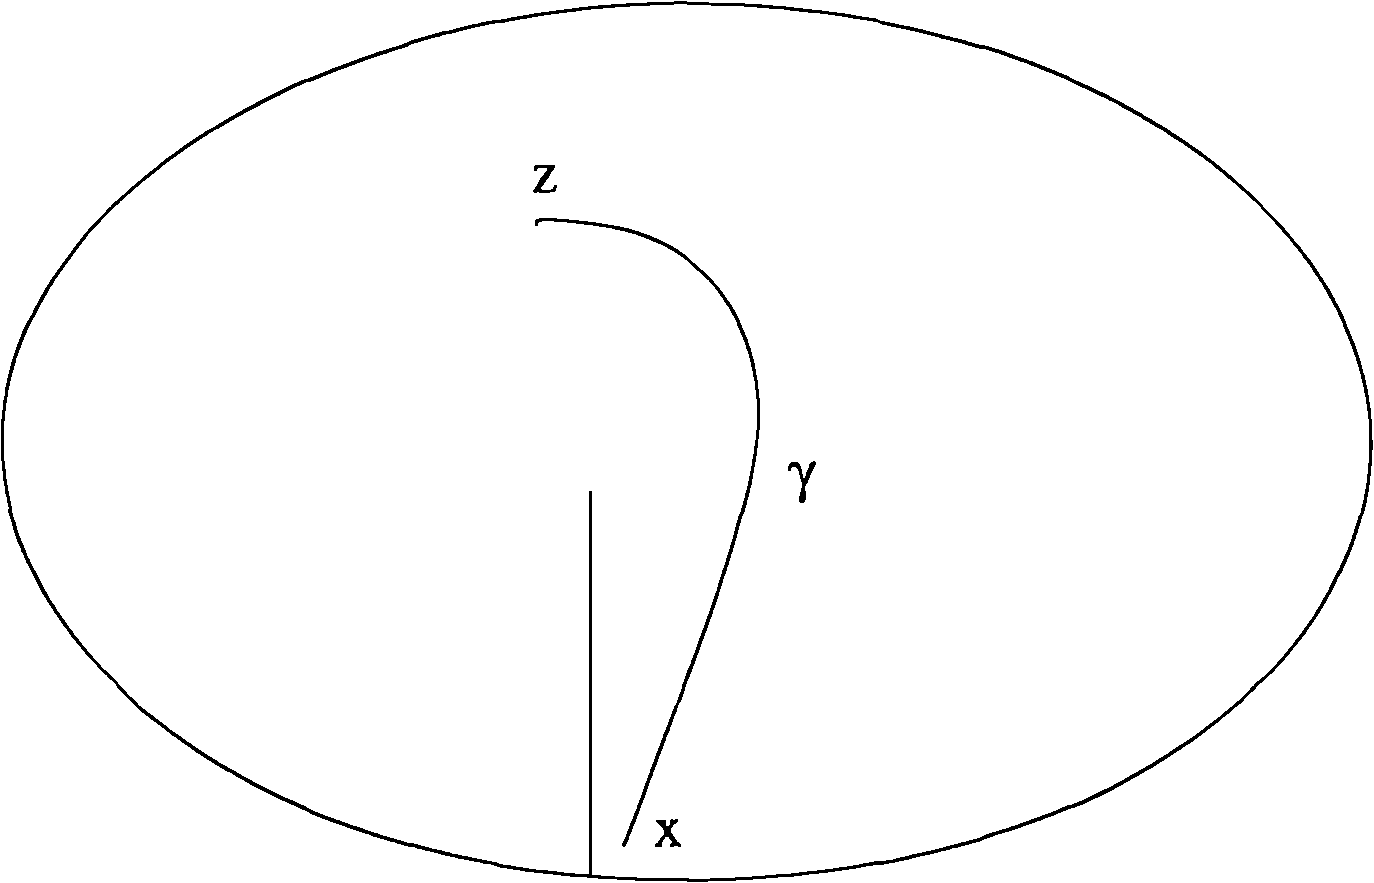
\includegraphics{Images/Img7.png}
    \bigskip
    \caption{A John domain.}
    \label{fig:ch3_1.3}
\end{figure}

\begin{definition}\label{def:ch3_1.11}
A domain $D$ is a John domain if there exist $z \in D$ and $c > 0$ such that for every $x \in D$ there is a rectifiable curve $\gamma$ connecting $x$ and $z$ in $D$ satisfying
\begin{equation}\label{eq:ch3_1.31}
    \dist(y,\partial D) \geq c\ell(\gamma(x,y)) \qquad \text{for all}~y \in \gamma,
\end{equation}
where $\ell(\gamma(x,y))$ is the length of the piece of the curve $\gamma$ between $x$ and $y$.
\end{definition}

A simple example of a John domain that is not a Lipschitz domain is simply the unit ball about $0$ minus the line segment from $0$ to $(0,\ldots,0,-1)$.

\index{John domain|)}

Returning to domains that are given locally as the region above the graph of a function, the boundary Harnack principle holds for H\"older domains of order $\alpha$ if $\alpha \in (0,1]$ (\cite{BanuelosBassyBurdzy1991}). A H\"older domain\index{Holder1@H\"older domain} is one where the domain looks locally like the region above the graph of a H\"older function\index{Holder2@H\"older function} of order $\alpha$; such a function is one where
\begin{equation}\label{eq:ch3_1.32}
    |\Gamma(z_1) - \Gamma(z_2)| \leq M_\Gamma|z_1 - z_2|^\alpha.
\end{equation}
In addition, in H\"older domains Brownian motion can be replaced by other diffusions, namely, ones corresponding to uniformly elliptic operators\index{Elliptic operator} of either divergence type or nondivergence type (\cite{BassBurdzy1991,BassBurdzy1994a}) (in the latter case, some regularity of the boundary is necessary when $\alpha \leq 1/2$). Even some degenerate elliptic operators are possible (\cite{Gao1993a}).

There are, however, examples of domains that are given locally as the region above the graph of a continuous function where the boundary Harnack principle does not hold (\cite{BassBurdzy1991}). It would be interesting to characterize those domains for which it holds.

The Fatou theorem\index{Fatou theorem} (see Sect.\ \chapref[III]{ch3_sec4}) says that in a Lipschitz domain a positive harmonic function has nontangential limits at almost every boundary point. This is not necessarily true in arbitrary domains. Yet the martingale convergence theorem says that $\lim_{t\to\tau_D}u(X_t)$ exists a.s.\ if $u$ is a positive harmonic function in $D$. This is, in some sense, a stochastic Fatou theorem valid in arbitrary domains. Might there be a stochastic version of the boundary Harnack principle that holds in every domain? A possible formulation would be: suppose $V$ is open, $K$ is compact contained in $V$, and $u$ and $v$ are two positive harmonic functions on $D$ that vanish on the regular points of $V \cap \partial D$ and are bounded in a neighborhood of $V \cap \partial D$. (See \cite{BassBurdzy1991} for a discussion of why these extra assumptions are necessary.) Does $\lim_{t\to\tau_D}(u/v)(X_t)$ remain bounded on the set $(X(\tau_D) \in K)$? To state this result for arbitrary domains, one really has to replace $\partial D$ by the Martin boundary of $D$. \cite{Doob1957} has shown that the limit exists $\P_z^x$-a.s., but here we need it to hold $\P_z^x$-a.s.\ for every $z \in K \cap \partial D$.

\mnewpage

\section{The Martin boundary for Lipschitz domains}\label{ch3_sec2}

\subsecbkm{ch3_sec2.1}{Martin boundary}

In this section we show that for a Lipschitz domain the Martin boundary\index{Martin boundary} is the same as the Euclidean boundary. This implies, for example, that Lipschitz domains have ``Poisson kernels'': there exists $M(x,z)$ such that every positive harmonic function $h$ in $D$ can be written $h(x) = \int_{\partial D} M(x,z)\mu(dz)$ for some $\mu$ supported on $\partial D$.

The main result can be stated as follows.

\begin{theorem}\label{thm:ch3_2.1}
Suppose $D$ is a Lipschitz domain. There exists a one-to-one mapping of the Martin boundary onto the Euclidean boundary. Each harmonic function corresponding to a Martin boundary point $z$ is minimal harmonic.
\end{theorem}

The first step is to show that the Martin boundary can be regarded as a subset of the Euclidean boundary. Fix $x_0 \in D$ and recall from Sect.\ \chapref[II]{ch2_sec7} that $M(x,y) = g_D(x,y)/g_D(x_0,y)$, $x,y \in D$. The Martin boundary is the set $\partial_M D = D^* - D$, where $D^*$ is the smallest compact set for which $M(x,y)$ is continuous in the extended sense in $y$. If we show $g_D(x,y)/g_D(x_0,y)$ is uniformly continuous in $y$ near the boundary of $D$, this will imply $D^* \subseteq \overline{D}$, and so we can identify the Martin boundary with a subset of the Euclidean boundary.

The oscillation\index{Oscillation} of a function $f$ on a set $A$ is defined by
\begin{equation}\label{eq:ch3_2.1}
    \Osc_A f = \sup_A f - \inf_A f.\index{OscA@$\Osc_A$}
\end{equation}

\begin{proposition}\label{prop:ch3_2.2}
$M(x,y)$ is uniformly continuous in $y$ for $y$ in a neighborhood of $\partial D$.
\end{proposition}

\begin{proof}
Fix $x_0$, $x \in D$. Pick $w \in \partial D$ and pick $r$ small enough so that $D \cap B(w,r)$ is the intersection of $B(w,r)$ with the region above the graph of a Lipschitz function. $r$ depends on $D$ but can be chosen to be independent of $w$. Fix a coordinate system as in the definition of Lipschitz domain. Pick $k_0$ large enough so that $Q(w,2^{-k_0},2^{-k_0}) \subseteq B(w,r)$ and $x,x_0 \not\in Q(w,2^{-k_0},2^{-k_0})$.

Write $Q_k = Q(w,2^{-k},2^{-k})$ and $h(y) = g_D(x_0,y)$. We want to show the oscillation of $g_D(x,\cdot)/h(\cdot)$ on $Q_{k+1}$ is controlled by the oscillation of $g_D(x,\cdot)/h(\cdot)$ on $Q_k$. Both $h$ and $g_D(x,\cdot)$ are harmonic functions on $D - \{x,x_0\}$ that vanish on $\partial D$. Moreover $g_D(x,y)$ and $h(y)$ are nonzero and finite for any $y \in Q_{k_0}$ by Harnack's inequality. By the boundary Harnack principle in $Q_k$ (see Exercise \ref{ex:ch3_11}), $g_D(x,\cdot)/h$ is bounded above and below by positive constants.

Fix $k$. Let $u(y) = Ag_D(x,y) + Bh(y)$, where $A$ and $B$ are real numbers so that
\mpagebreak
\[
    \sup_{Q_k}(u/h) = 1, \qquad \inf_{Q_k}(u/h) = 0.
\]
Clearly $u$ is harmonic in $Q_k$, and
\[
    \Osc_{Q_k}(u/h) = \sup_{Q_k}(u/h) - \inf_{Q_k}(u/h) = 1.
\]
Pick $z_k \in U(w,2^{-k},2^{-k})$. If $u(z_k)/h(z_k) \leq 1/2$, replace $u$ by $h-u$. So we may suppose $u(z_k)/h(z_k) \geq 1/2$ and still have $\sup_{Q_k}(u/h) = 1$, $\inf_{Q_k}(u/h) = 0$, and $u$ harmonic in $Q_k$.

By the boundary Harnack principle, if $y \in Q_{k+1}$,
\[
    (u/h)(y) \geq c_1(u/h)(z_k) \geq c_1/2.
\]
So
\[
    \Osc_{Q_{k+1}}(u/h) \leq 1-c_1/2 = \rho.
\]
Letting $\rho = 1-c_1/2$ and undoing the algebra,
\[
    \Osc_{Q_{k+1}}(g_D(x,y)/h(y)) \leq \rho \Osc_{Q_k}(g_D(x,y)/h(y)),
\]
and $\rho < 1$.

$g_D(x,y)/h(y)$ is bounded by $c_2$ on $Q_{k_0}$ by the boundary Harnack principle. So $\Osc_{Q_{k+1}}(g_D(x,y)/h(y)) \leq c_2\rho^{k-k_0}$, or
\[
    \Big|\frac{g_D(x,y)}{h(y)} - \frac{g_D(x,y')}{h(y')}\Big| \leq c_3\rho^k
\]
if $y,y' \in Q(w,2^{-k},2^{-k})$. This and Exercise \ref{ex:ch3_12} imply the uniform H\"older continuity of $g_D(x,y)/h(y)$, which implies our result.
\end{proof}

As a consequence, if $y \to z \in \partial D$, $g_D(x,y)/g_D(x_0,y) = M(x,y)$ converges. Call the limit $M(x,z)$. We next want to show that if $z_1 \neq z_2$, then $M(\cdot,z_1) \neq M(\cdot,z_2)$. This will imply that each Euclidean boundary point corresponds to a different positive harmonic function, hence the Martin boundary cannot be identified with a proper subset of the Euclidean boundary.

\begin{proposition}\label{prop:ch3_2.3}
If $M(\cdot,z_1) \equiv M(\cdot,z_2)$ for $z_1,z_2 \in \partial D$, then $z_1 = z_2$.
\end{proposition}

\begin{proof}
First we want to show $M(\cdot,z)$ vanishes on $D - \{z_1\}$. Fix $y_0 \in D$, $y_0 \neq x_0$. Suppose $w \in \partial D$, $w \neq z_1$. Since $g_D(x,y_0) \to 0$ as $x \to w$, given $\epsilon$ there exists $\delta < |w-z_1|/4$ such that $g_D(x,y_0) \leq \epsilon$ if $|x-w| \leq \delta$. Then by the boundary Harnack principle in $D - (B(x,\delta/2) \cup B(x_0,\delta/2))$ (see Exercise \ref{ex:ch3_9}),
\[
    \frac{g_D(x,y)}{g_D(x_0,y)} \leq \frac{cg_D(x,y_0)}{g_D(x_0,y_0)} \leq \frac{c\epsilon}{g_D(x_0,y_0)}
\]
if $|x-w| \leq \delta$. Letting $y \to z_1$, we see that $M(x,z_1) \leq c\epsilon/g_D(x_0,y_0)$. Since $\epsilon$ is arbitrary, $M(x,z_1) \to 0$ as $x \to w \neq z_1$. Moreover the convergence is uniform on compact subsets of $\partial D - \{z_1\}$.

The next step is to show that there is only one $\mu$ supported on $\partial D$ such that $M(x,z_1) = \int M(x,w)\mu(dw)$, namely, $\mu = \delta_{z_1}$. If we show this, then the same argument for $z_2$ will tell us that if $M(x,z_1) \equiv M(x,z_2)$, then $\delta_{z_1} = \mu = \delta_{z_2}$, or $z_1 = z_2$.

So suppose $M(x,z_1) = \int_{\partial D} M(x,w)\mu(dw)$, $\mu \neq \delta_{z_1}$. Since $M(x_0,w) = 1$ for all $w$, $1 = M(x_0,z_1) = \mu(\partial D)$. If $\mu \neq \delta_{z_1}$, there exists $\epsilon$ such that $\mu_\epsilon = \mu|_{B(z_1,\epsilon)^c} \neq 0$. Then $\int M(x,w)\mu_\epsilon(dw)$ is a harmonic function bounded above by $M(x,z_1)$.

Now the first paragraph of the proof showed that if $|w-z_1| \geq \epsilon$, then $M(x,w) \to 0$ (uniformly) as $x \to w' \in \partial D \cap B(z_1,\epsilon/2)$. So $\int M(x,w)\mu_\epsilon(dw) \to 0$ as $x \to w' \in \partial D \cap B(z_1,\epsilon/2)^c$. On the other hand, if $x \to w' \in \partial D \cap B(z_1,\epsilon/2)$, then
\[
    \int M(x,w)\mu_\epsilon(dw) \leq \int M(x,w)\mu(dw) = M(x,z_1) \to 0.
\]
By the maximum principle, $\int M(x,w)\mu_\epsilon(dw) = 0$. The boundary Harnack principle tells us that $g_D(x,y)/g_D(x_0,y)$ stays bounded below by a positive constant as $y \to \partial D$. Therefore $M(x,w)$ is positive for all $w$, hence $\mu_\epsilon = 0$. Since $\epsilon$ is arbitrary, $\mu(\{z_1\}^c) = 0$. Because $\mu(\partial D) = 1$, we have $\mu = \delta_{z_1}$ as desired.
\end{proof}

The proof of Theorem \ref{thm:ch3_2.1} will be complete once we prove the following.

\begin{proposition}\label{prop:ch3_2.4}
For each $z \in \partial D$, $M(x,z)$ is minimal harmonic.\index{Minimal harmonic function}
\end{proposition}

\begin{proof}
Suppose $h(x) \leq M(x,z)$ in $D$. We can write $h(x) = \int M(x,w)\mu(dw)$ for some $\mu$ supported on $\partial D$, and by exactly the same argument as the one in the proof of Proposition \ref{prop:ch3_2.3}, we deduce that $\mu(\{z\}^c) = 0$. Therefore $\mu = c\delta_z$ for some $c$.
\end{proof}

\subsecbkm{ch3_sec2.2}{Harmonic measure}
\index{Harmonic measure|(}

We want to show that the Martin kernel is the density of harmonic measure with respect to two different starting points.

\begin{definition}\label{def:ch3_2.5}
The harmonic measure of a set $A \subseteq \partial D$ is defined by
\begin{equation}\label{eq:ch3_2.2}
\omega^x(A) = \omega(x,A) = \P^x(X_{\tau_D} \in A).
\end{equation}
\end{definition}

For each $A$, $\omega(x,A)$ is a harmonic function, and so by the usual Harnack inequality, $\omega(x,A) \leq c\omega(x_0,A)$ for some $c$ independent of $A$. Hence $\omega(x,\cdot)$ is absolutely continuous with respect to $\omega(x_0,\cdot)$ with a Radon-Nikodym derivative that is bounded by $c$.

\begin{theorem}\label{thm:ch3_2.6}
\[
    \omega(x,A) = \int_A M(x,w)\omega(x_0,dw).
\]
\end{theorem}

\begin{proof}
Let $R(x,y)$ be the Radon-Nikodym derivative of $\omega(x,dy)$ with respect to $\omega(x_0,dy)$. Fix $y \in \partial D$. For each $k$, let $Q_{yk}$ denote the cube of the form
\[
    [j_1/2^k,(j_1+1)/2^k] \times \cdots \times [j_d/2^k,(j_d+1)/2^k]
\]
that contains $y$, where $j_1,\ldots,j_d$ are integers.
\[
    h_k(x) = \frac{\omega(x,Q_{yk} \cap \partial D)}{\omega(x_0,Q_{yk} \cap \partial D)}
\]
(with the convention $0/0 = 0$) is a harmonic function on $D - Q_{yk}$. Since $h_k(x_0) = 1$, the Harnack inequality shows that for any $k_0$, if $k > k_0$, then $h_k$ is bounded on any subdomain $D'$ of $D - Q_{y,k_0}$, uniformly over $k > k_0$. By Corollary \chapref[II]{cor:ch2_1.4}, the $h_k$, $k > k_0$, are equicontinuous on subdomains $D''$ of $D'$, so a subsequence converges to a harmonic function on $D''$. By a diagonalization procedure, we can find a subsequence of $h_k$ that converges to a harmonic function, call it $h$, uniformly on compact subsets of $D$.

$h(x) = \int M(x,w)\mu(dw)$ for some $\mu$ supported on $\partial D$. Now we know each $h_k$ is bounded on subdomains $D'$ and clearly it vanishes continuously on $\partial D - Q_{y,k-1}$. So by the Carleson estimate (Theorem \ref{thm:ch3_1.8}) and Lemma \ref{lem:ch3_1.9}, we see that $h_k(x) \to 0$ as $x \to z \in \partial D - Q_{y,k-1}$, uniformly over such $z$. Hence $h(x) \to 0$ as $x \to z \in \partial D - \{y\}$. By the argument of Proposition \ref{prop:ch3_2.3}, $\mu(\{y\}^c) = 0$, or $\mu = c\delta_y$. Since $h_k(x_0) = 1$, then $c = 1$. Therefore $h(x) = M(x,y)$.

Except for a set of $y$s in an $\omega(x_0,\cdot)$ null set,
\begin{equation}\label{eq:ch3_2.3}
    \lim_{k \to \infty} \frac{\omega(x,Q_{yk} \cap \partial D)}{\omega(x_0,Q_{yk} \cap \partial D)} = R(x,y)
    % Note: changed "k\to 0" in the limit on the RHS
\end{equation}
by Exercise \ref{ex:ch3_13}. So $M(x,y) = R(x,y)$, a.e. Therefore $M(x,y)$ is also a Radon-Nikodym derivative of $\omega(x,\cdot)$ with respect to $\omega(x_0,\cdot)$, and the theorem follows.
\end{proof}

\index{Harmonic measure|)}

\subsecbkm{ch3_sec2.3}{h-path transforms}

Let $(\P_z^x,X_t)$ denote the $h$-path transform of Brownian motion killed on exiting $D$ by the harmonic function $M(\cdot,z)$, that is,
\begin{equation}\label{eq:ch3_2.4}
    \P_z^x(\cdot) = \P_{M(\cdot,z)}^x(\cdot).\index{P4@$\P_z^x$}
\end{equation}
\mnewpage
The next proposition shows that $(\P_z^x,X_t)$ can be interpreted as Brownian motion conditioned to exit $D$ at $z$. For the reader interested only in the case where $D$ is a ball or half-space, replace $M(\cdot,z)$ everywhere by the Poisson kernel with pole at $z$.

\begin{proposition}\label{prop:ch3_2.7}
If $A \in \FC_{\tau_D}$,
\[
    \int_B \P_z^x(A)\P^{x_0}(X_{\tau_D} \in dz) = \P^{x_0}(X_{\tau_D} \in B; A).
\]
\end{proposition}

\begin{proof}
Suppose $D_n$ are subdomains increasing up to $D$ (that is, $\overline{D}_n \subseteq D_{n+1}$, $\cup_n D_n = D$) and $A \in \FC_{\tau_{D_n}}$. Then
\begin{align*}
    \int_B \P_z^x(A)\P^{x_0}(X_{\tau_D} \in dz) &= \int_B \frac{\E^{x_0}[M(X_{\tau_{D_n}},z); A]}{M(x_0,z)} \P^{x_0}(X_{\tau_D} \in dz) \\
    &= \E^{x_0}\Big[\int_B M(X_{\tau_{D_n}},z) \P^{x_0}(X_{\tau_D} \in dz); A\Big]
\end{align*}
since $M(x_0,z) = 1$. By Theorem \ref{thm:ch3_2.6} and the strong Markov property, this is equal to
\[
    \E^{x_0}\big[\P^{X(\tau_{D_n})}(X_{\tau_D} \in B); A\big] = \P^{x_0}(X_{\tau_D} \in B; A).
\]
This proves the lemma for $A \in \FC_{\tau_{D_n}}$, and a linearity and limiting argument gives it for $A \in \FC_{\tau_D}$.
\end{proof}

We will need a zero-one law\index{Zero-one law} due to Brossard; \cite[see][pp.~102-104]{Durrett1984}.

\begin{definition}\label{def:ch3_2.8}
$A$ is shift invariant\index{Shift invariant event} if whenever $S < \tau_D$ is a stopping time, $1_A \circ \theta_S = 1_A$, $\P^x$-a.s.\ for every $x \in D$.
\end{definition}

Roughly, $A$ is shift invariant if for each $\epsilon$, $A$ depends on $X_t$, $\tau_D - \epsilon < t < \tau_D$. For example, $(\lim_{t\to\tau_D} u(X_t)~\text{exists})$ and $(\lim_{t\to\tau_D} u(X_t) > B)$ are shift invariant, but $(\sup_{t<\tau_D} u(X_t) > B)$ is not.

\begin{theorem}\label{thm:ch3_2.9}
If $A$ is shift invariant, then $x \to \P_z^x(A)$ is constant and is either identically $0$ or identically $1$.
\end{theorem}

It is not true, in general, that $z\to \P_z^x(A)$ is constant. For example, the second example of a shift invariant set given above does not have this property.

\begin{proof}
Let $k(x) = \P_z^x(A)$, $S < \tau_D$. Then
\[
    k(x) = \P_z^x(A) = \P_z^x(A \circ \theta_S) = \E_z^x\E_z^{X_S}(A) = \E_z^xk(X_S).
\]
\mnewpage
So $k(x) = \E_z^xM(X_S,z)k(X_S)/M(x,z)$, or $M(\cdot,z)k(\cdot)$ is harmonic. It is clearly nonnegative and bounded by $M(\cdot,z)$ since $k \leq 1$. Since $M(\cdot,z)$ is a minimal harmonic function, $M(\cdot,z)k$ is a constant multiple of $M(\cdot,z)$, or $k$ is identically constant.

If $D_n$ are subdomains increasing to $D$ and $B \in \FC_{\tau_{D_n}}$,
\begin{align*}
    \P_z^x(A \cap B) &= \P_z^x(A \circ \theta_{\tau_{D_n}} \cdot B)  = \E_z^x\big[\P_z^{X(\tau_{D_n})}(A); B\big] \\
    &= \E_z^x[k(X_{\tau_{D_n}});B] \\
    &= k(x)\P_z^x(B) \\
    &= \P_z^x(A)\P_z^x(B),
\end{align*}
since $k$ is constant. So $\P_z^x(A \cap B) = \P_z^x(A)\P_z^x(B)$ for $B \in \FC_{\tau_{D_n}}$. This is true for all $n$, so it is true for $B\in \FC_{\tau_D}$. Now let $B = A$, or $\P_z^x(A) = [\P_z^x(A)]^2$, hence $\P_z^x(A)$ is $0$ or $1$.
\end{proof}

The zero-one law is not surprising if it is viewed as follows. The law of $X_{\tau_D-t}$ under $\P_z^x$ can be shown to be the same as the law of Brownian motion started at $z$ and conditioned to go to $x$ before exiting $D$ (see \cite{Williams1979}, \cite{ChungWalsh1969}, and Exercise \ref{ex:ch3_14}). Shift invariant events are in $\FC_{0+}$ for the time-reversed process. The analog of Corollary \chapref[I]{cor:ch1_3.6} holds for $h$-path transforms of Brownian motion (the same proof works), so events in $\FC_{0+}$ have probability $0$ or $1$.

\subsecbkm{ch3_sec2.4}{Extensions}

Since the equivalence of the Martin boundary and the Euclidean boundary follows from the boundary Harnack principle, and since the boundary Harnack principle holds in H\"older domains, one might expect that the results of this section hold for H\"older domains. That is not the case. The problem is that the constant $c_1$ in Proposition \ref{prop:ch3_2.2} now depends on $k$. One can show that the Martin boundary equals the Euclidean boundary for domains a little less regular than Lipschitz domains, namely, $C^\gamma$\index{C2@$C^\gamma$} domains, where $\gamma(x) \leq ax\log\log(1/x)/\log\log\log(1/x)$, provided $a$ is sufficiently small (\cite{BassBurdzy1993}). A $C^\gamma$ domain is one that looks locally like the region above the graph of a $C^\gamma$ functions, and a $C^\gamma$ function $\Gamma$ is one where $|\Gamma(x)-\Gamma(y)| \leq \gamma(|x-y|)$.

A probabilist would see the above expression for $\gamma$ and assume that the ``right'' theorem is one where $\gamma_c(x) = cx\log\log(1/x)$ for some $c$. That also is incorrect: for any $c$ there exist domains above the graph of a $C^{\gamma_c}$ function for which the Martin boundary is larger than the Euclidean boundary (\cite{BassBurdzy1993}).

Besides domains above the graphs of functions, there are other situations where the Martin boundary has been determined. \cite[See][]{Ancona1987}.

\mpagebreak

A Denjoy domain\index{Denjoy domain} $D$ is a subset of $\R^2$ such that $D^c$ is a subset of the $x$-axis. Each point on $\partial D$ is known to be either one or two Martin boundary points. A criterion is known for such domains together with results for similar sectorial domains (\cite{CranstonSalisbury1993}). Given an arbitrary domain $D$ and $z \in \partial D$, can one give a condition on whether $z$ corresponds to more than one Martin boundary point? What about domains above the graph of a function? Presumably any such condition would be in terms of capacities or the solutions to certain simpler Dirichlet problems. \cite{Bishop1992} discusses some related problems.

\section{The conditional lifetime problem}\label{ch3_sec3}

\subsecbkm{ch3_sec3.1}{Formulation}

The conditional lifetime problem is this: if one has a bounded domain $D$ and $h$ is positive and harmonic on $D$, is $\E_h^x\tau_D < \infty$? Here $\E_h^x$ is the expectation of Brownian motion $h$-path transformed by the harmonic function $h$ and $\tau_D$ is the time of exiting $D$. We will show that the answer is yes if $D$ is a bounded domain in $\R^2$ or if $D$ is a Lipschitz domain in $\R^d$.

This problem looks like a purely probabilistic problem with little interest to analysts. Although we give an equivalent analytic formulation, strictly speaking this is true. However, the proof we give, with a few minor modifications, also shows that Lipschitz domains are intrinsically ultracontractive (which implies all sorts of interesting things about the fundamental solution to the heat equation on $D$ with Dirichlet boundary conditions) and that the parabolic boundary Harnack principle holds (which is the boundary Harnack principle for the heat equation); see the Extensions subsection.

The condition $\E_h^x\tau_D < \infty$ can be rewritten as follows. Let $D_n$ be subdomains increasing to $D$. This means that $D_n$ are domains such that $\overline{D}_n \subseteq D_{n+1}$ and $\cup_nD_n = D$. If $\E_h^x\tau_D < \infty$,
\begin{align*}
    \infty &> c \geq \E_h^x \int_0^{\tau_{D_n}} 1_{D_n}(X_s)ds \\
    &= \E^x\Big[h(X(\tau_{D_n})) \int_0^{\tau_{D_n}} 1_{D_n}(X_s)ds\Big]/h(x) \\
    &= \E^x\Big[\int_0^\infty 1_{(s<\tau_{D_n})}\E^x[h(X_{\tau_{D_n}})|\FC_s]1_{D_n}(X_s)ds\Big]/h(x) \\
    &= \E^x\Big[\int_0^{\tau_{D_n}} h(X_s)1_{D_n}(X_s)ds\Big]/h(x) \\
    &= \int_{D_n} g_{D_n}(x,y)h(y)dy/h(x).
\end{align*}
\mnewpage
To obtain the next to the last identity, we used the fact that $h(X_{s\wedge\tau_D})$ is a martingale. Letting $n \to \infty$,
\[
    \int_{D_n} g_{D_n}(x,y)h(y)dy \uparrow \int_D g_D(x,y)h(y)dy,
\]
and so the condition $\E_h^x\tau_D < \infty$ is equivalent to
\[
    \int_D g_D(x,y)h(y)dy/h(x) < \infty.
\]

Before proceeding to the proof of the main results, let us prove a simple estimate on simple random walks, well known to probabilists (\cite{Feller1968}). Suppose $Y_i = +1$ with probability $p$, $-1$ with probability $1-p$, the $Y_i$ are independent, and $Z_n = Z_0 + \sum_{i=1}^n Y_i$. Let $\P^j$ denote the law of $Z$ given that $Z_0 = j$.

\begin{proposition}\label{prop:ch3_3.1}
If $p > 1/2$, then $\E^j \sum_{n=0}^\infty 1_{\{k\}}(Z_n) \leq c < \infty$, $c$ independent of $j$ and $k$.
\end{proposition}

\begin{proof}
By Exercise \ref{ex:ch3_26}, $\P^1(Z_k~\text{ever hits}~0) \leq \rho < 1$. So
\begin{align*}
    \P^0(Z_k~\text{hits}~0~\text{for some}~k > 0) &= \P^0(Z_1 = 1, Z_k~\text{hits}~0~\text{for some}~k > 0) \\
    &\qquad + \P^0(Z_1 = -1) \\
    &\leq p\rho + (1-p) = \rho'.
\end{align*}
By the strong Markov property,
\[
    \P^0(Z_k~\text{hits}~0~\text{at least twice}) \leq (\rho')^2,
\]
and similarly for hitting $0$ three times, etc. Therefore
\begin{align*}
    \E^0 \sum_{k=0}^\infty 1_{\{0\}}(Z_k) &\leq 1 + \E^0 \sum_{i=1}^\infty i\P^0(Z_k~\text{hits}~0~\text{at least}~i~\text{times}) \\
    &\leq 1 + \sum_{i=1}^\infty i(\rho')^i < \infty.
\end{align*}
By the strong Markov property,
\[
    \E^{j-k} \sum_{n=0}^\infty 1_{\{0\}}(Z_n) \leq \E^0 \sum_{n=0}^\infty 1_{\{0\}}(Z_n),
\]
and our result follows by translation invariance.
\end{proof}

\mpagebreak

\subsecbkm{ch3_sec3.2}{Lipschitz domains}

Let $D$ be a Lipschitz domain. Fix $x_0 \in D$. Let $h$ be a positive harmonic function on $D$. Since $\P_{ch}^x = \P_h^x$, we may normalize $h$ so that $h(x_0) = 1$. For $n \in \Z$, let
\begin{equation}\label{eq:ch3_3.1}
    L_n = \{x \in D : h(x) = 2^n\}, \quad R_n = \{x \in D : 2^{n-1} \leq h(x) \leq 2^{n+1}\}.
    % Note: \quad is used here.
\end{equation}
The main estimate we need is the following.

\begin{theorem}\label{thm:ch3_3.2}
There exist $c > 0$ and $\alpha > 1$ (depending on $D$ but not $n$ or $x$) such that
\[
    \E^x\tau_{R_n} \leq c(1 + |n|)^{-\alpha}.
\]
\end{theorem}

\begin{proof}
Since $D$ is bounded, $D \subseteq B(x,M)$ for $M = 2\diam(D)$, hence
\begin{equation}\label{eq:ch3_3.2}
    \E^x\tau_{R_n} \leq \E^x\tau_{B(x,M)} \leq c(\diam(D))^2
\end{equation}
(see Exercise \chapref[II.8]{ex:ch2_17}). So it suffices to obtain the estimate for $|n|$ large.

Suppose $|n|$ is large but $n$ is negative. Let $S_n = \{x : h(x) < 2^{n+2}\}$. Clearly $R_n \subseteq S_n$, so $\tau_{R_n} \leq \tau_{S_n}$. Recall $h(x_0) = 1$. Now by Lemma \ref{lem:ch3_1.9}, there exists $\beta$ such that if $h(x) \leq 2^{n+2}$, then $\dist(x,\partial D) \leq c(2^{n+2})^\beta$. Let $r_n = c2^{(n+2)\beta}$. Hence $S_n \subseteq \{x : \dist(x,\partial D) \leq r_n\}$.

$S_n$ is typically a thin strip and we argue that Brownian motion cannot go very long before exiting this strip. If $V_0 = 0$, $V_1 = \inf\{t : |X_t-X_0| \geq cr_n\}$ and $V_{i+1} = V_i + V_1 \circ \theta_{V_i}$, then
\[
    \sup_{z\in S_n} \P^z(V_1 \leq \tau_{S_n}) \leq \rho < 1,
\]
just as in Lemma \ref{lem:ch3_1.5}. Hence, as in Lemma \ref{lem:ch3_1.5}, $\P^y(V_j < \tau_{S_n}) \leq \rho^j$. Now
\begin{align}\label{eq:ch3_3.3}
    \E^x\tau_{S_n} &= \sum_{j=0}^\infty \E^x[\tau_{S_n}; V_{j+1} > \tau_{S_n} \geq V_j] \\
    &\leq \sum_{j=0}^\infty \E^x[V_{j+1}; V_{j+1} > \tau_{S_n} \geq V_j] \notag \\
    &\leq \sum_{j=0}^{\infty} \sum_{i=0}^j \E^x[V_{i+1} - V_i; V_{j+1} > \tau_{S_n} \geq V_j] \notag \\
    &= \sum_{i=0}^{\infty} \sum_{j=i}^{\infty} \E^x[V_{i+1} - V_i; V_{j+1} > \tau_{S_n} \geq V_j] \notag \\
    &\leq \sum_{i=0}^{\infty} \E^x[V_1 \circ \theta_i; \tau_{S_n} \geq V_i] = \sum_{i=0}^{\infty} \E^x\big[\E^{X_{V_i}}V_1; \tau_{S_n} \geq V_i\big ] \notag \\
    &\leq c\sum_{i=0}^{\infty} cr_n^2\rho^i \leq cr_n^2. \notag
\end{align}
\mnewpage
This gives our result for such $n$ with a great deal to spare.

For $n$ large and positive, the proof is similar after observing that by Lemma \ref{lem:ch3_1.9} there exists $\beta$ such that $h(x) \geq 2^{n-2}$ implies that $\dist(x,\partial D) \leq c2^{-(n-2)\beta}$.
\end{proof}

We can now prove the following.

\index{Conditional lifetime theorem|(}

\begin{theorem}\label{thm:ch3_3.3}
There exists $c$, depending only on $D$ and not $h$ or $x$, such that $\E_h^x\tau_D \leq c$.
\end{theorem}

\begin{proof}
Let $S_0 = \inf\{t : X_t \in \cup_nL_n\}$, $W_i$ the integer $n$ such that $X_{S_i} \in L_n$, and $S_{i+1} = \inf\{t > S_i : X_t \in \cup_nL_n - L_{W_i}\}$. The $S_i$s are successive hits to different $L_n$s and the $W_i$s are which $L_n$s are hit.

% Note: changed Proposition 3.2 to Theorem 3.2

Let $v_n = \sup_{y\in L_n} \E_h^yS_1$. Let us use Theorem \ref{thm:ch3_3.2} to obtain a bound on $v_n$. We have
\[
    v_n = \sup_{y\in L_n} \frac{\E^y[S_1h(X_{S_1})]}{h(y)}.
\]
If $y \in L_n$, then $h(y) = 2^n$ and $X_{S_1} \in L_{n+1}$ or $L_{n-1}$; hence $h(X_{S_1}) \leq 2^{n+1}$. Therefore
\[
    v_n \leq \sup_{y\in L_n} 2\E^yS_1 \leq \sup_{y\in R_n} 2\E^y\tau_{R_n} \leq c(1 + |n|)^{-\alpha}.
\]

Next we bound $\E_h^x\tau_D$ in terms of $v_n$ and the number of visits to $L_n$. Since $X_t \to \partial D$, $\P_h^x$-a.s.,
\[
    \E_h^x\tau_D = \E_h^x \sum_{i=0}^\infty (S_{i+1} - S_i).
\]
We then write
\begin{align}\label{eq:ch3_3.4}
    \E_h^x\tau_D &= \E_h^x \sum_{i=0}^\infty \E_h^{X_{S_i}}(S_1) \leq \E_h^x \sum_{i=0}^\infty v_{W_i} \\
    &= \E_h^x \sum_{n=-\infty}^\infty \sum_{i=0}^\infty v_n1_{L_n}(X_{S_i}) = \E_h^x \sum_{n=-\infty}^\infty v_nN_n, \notag
\end{align}
where $N_n = \sum_{i=0}^\infty 1_{L_n}(X_{S_i})$ is the number of times that $X_{S_i} \in L_n$.

Since $h$ is harmonic, $h(X_t)$ is a martingale. Hence if $x \in L_n$, the $\P^x$ probability of hitting $L_{n+1}$ before $L_{n-1}$ is, by Corollary \chapref[I]{cor:ch1_4.10},
\[
    (2^n - 2^{n-1})/(2^{n+1} - 2^{n-1}) = 1/3.
\]
Therefore
\begin{align*}
    \P_h^x(T_{L_{n+1}} < T_{L_{n-1}}) &= \frac{\E^x\big[h(X(T_{L_{n+1}} \wedge T_{L_{n-1}})); T_{L_{n+1}} < T_{L_{n-1}}\big]}{h(x)} \\
    % Note: added missing ) in the first line
    &= \frac{2^{n+1}\P^x(T_{L_{n+1}} < T_{L_{n-1}})}{2^n} = \frac{2}{3}.
\end{align*}
\mnewpage
Similarly $\P_h^x(T_{L_{n-1}} < T_{L_{n+1}}) = 1/3$ for $x \in L_n$. So, under $\P_h^x$, $W_i$ is a simple random walk with $p = 2/3$, $1-p = 1/3$. By Proposition \ref{prop:ch3_3.1}, $\E_h^xN_n \leq c < \infty$. Substituting in \eqref{eq:ch3_3.4},
\[
    \E_h^x\tau_D \leq \sum_{n=-\infty}^\infty v_n\E_h^xN_n \leq c \sum_{n=-\infty}^\infty (1 + |n|)^{-\alpha} < \infty.
\]
This completes the proof.
\end{proof}

\subsecbkm{ch3_sec3.3}{The two-dimensional case}

% Note: changed Proposition 3.2 to Theorem 3.2 in the next paragraph.

For the $d = 2$ result, what is different is Theorem \ref{thm:ch3_3.2}. As we shall see, once we have the following replacement, the Cranston-McConnell result follows quickly.

\begin{theorem}\label{thm:ch3_3.4}
Suppose $D \subseteq \R^2$ is bounded. Then there exists $c$ depending on $D$ but not $n$ or $x$ such that $\E^x\tau_{R_n} \leq c|R_n|$.
\end{theorem}

\begin{proof}
Suppose $|R_n| = r^2$. Fix $x \in R_n$, and note $|B(x,2r) - R_n| \geq r^2/2$. Let $B = B(x,3r)$, $A = B(x,2r) - R_n$. By the explicit formula for $g_B$ (Exercise \chapref[II.8]{ex:ch2_45}), there exists $c_1$ such that $g_B(x,y) \geq c_1$ on $B(x,2r)$. So
\begin{align*}
    c_1r^2/2 &\leq c_1|A| \leq \int g_B(x,y)1_A(y)dy = \E^x \int_0^{\tau_B} 1_A(X_s)ds \\
    &= \E^x\Big[\E^{X_{T_A}} \int_0^{\tau_B} 1_A(X_s)ds; T_A < \tau_B\Big] \\
    &\leq \big(\sup_{y\in B} \E^y\tau_B\big)\P^x(T_A < \tau_B) \\
    &\leq c_2r^2\P^x(T_A < \tau_B).
\end{align*}
Therefore $\P^x(T_A < \tau_B) \geq c_1/2c_2$. To leave $B$ before leaving $R_n$, the process must leave $B$ before hitting $A$, or $\P^x(\tau_{R_n} > \tau_B) \leq 1 - c_1/2c_2 = \rho$.

We now write:
\begin{align*}
    \E^x\tau_{R_n} &\leq \E^x\tau_B + \E^x[\tau_{R_n} - \tau_B; \tau_{R_n} > \tau_B] \\
    &\leq cr^2 + \E^x[\E^{X_{\tau_B}}\tau_{R_n}; \tau_{R_n} > \tau_B] \\
    &\leq cr^2 + (\sup_{y} \E^y\tau_{R_n})\P^x(\tau_{R_n} > \tau_B) \\
    &\leq cr^2 + M\rho,
\end{align*}
where $M = \sup_y \E^y\tau(R_n)$. Taking a supremum over $x$, we see $M \leq cr^2 + M\rho$. Since $D$ is bounded, $M < \infty$, and therefore
\[
    M \leq cr^2/(1-\rho) \leq c|R_n|.
\]
\end{proof}

\begin{theorem}\label{thm:ch3_3.5}
If $D \subseteq \R^2$ is bounded, there exists $c$ independent of $x$ and $h$ such that $\E_h^x\tau_D \leq c$.
\end{theorem}

\begin{proof}
We follow the proof of Theorem \ref{thm:ch3_3.3} almost exactly, except that here $v_n \leq c|R_n|$. Since
\[
    \sum_{n=-\infty}^{\infty} v_n \leq c \sum_{n=-\infty}^{\infty} |R_n| \leq c|D| < \infty,
\]
our result follows.
\end{proof}

\index{Conditional lifetime theorem|)}

\subsecbkm{ch3_sec3.4}{Extensions}

It is clear from the estimate $(2^{-|n|})^\beta \leq c(1 + |n|)^{-\alpha}$ that things can be improved greatly. In fact, for $d \geq 3$, the expected lifetime can be bounded by a constant depending only on $D$ for domains that are given locally as the region above a continuous function, and even much worse (see \cite{Davis1991}, \cite{Banuelos1991,Banuelos1992}, and \cite{BassBurdzy1992}). It is not true, however, that the expected lifetime of conditional Brownian motion is finite for every bounded domain in $\R^d$, $d \geq 3$; see \cite{CranstonMcConnell1983}. In $d = 2$, domains with infinite area can still have finite expected lifetime; see, e.g., \cite{Xu1991}, \cite{BanuelosDavis1992}.

In addition to conditional Brownian motion, one can also work with conditioned diffusions, where the diffusions are associated to various sorts of elliptic operators\index{Elliptic operator} (\cite{BassBurdzy1992}, \cite{Banuelos1991,Banuelos1992}, \cite{Gao1993b}).

% Note: changed \int_0^{\tau_d} to \int_0^{\tau_D} in the next paragraph.

Since $\tau_D = \int_0^{\tau_D} 1(X_s)ds$ is an additive functional with bounded potentials, then by Theorem \chapref[I]{thm:ch1_6.11}, $\tau_D$ actually has moments of all orders and even exponential moments. So by Chebyshev's inequality, $\P_h^x(\tau_D > t) \leq c_1\exp(-c_2t)$. An explicit value for $c_2$ is known; see \cite{BanuelosDavis1989}.

These exponential estimates are just one example of what one can say if the domain $D$ is intrinsically ultracontractive\index{Intrinsically ultracontractive}. A domain $D$ is intrinsically ultracontractive if there exists a positive eigenfunction $\varphi$ of the Laplacian in $D$ with Dirichlet boundary conditions (i.e., $\varphi = 0$ on the points of $\partial D$ regular for $D^c$, $\varphi \geq 0$ on $D$, and $\Delta\varphi = \lambda\varphi$ in $D$ for some $\lambda$) and constants $c_1(t)$ and $c_2(t)$ such that
\[
    c_1(t)\varphi(x)\varphi(y) \leq p_D(t,x,y) \leq c_2(t)\varphi(x)\varphi(y).
\]
This concept, introduced by \cite{DaviesSimon1984}, leads to very strong estimates of $p_D(t,x,y)$, the transition density of Brownian motion killed on exiting $D$ (equivalently, the fundamental solution of the heat equation on $D$ with Dirichlet boundary conditions).

It turns out that being intrinsically ultracontractive is equivalent to the parabolic boundary Harnack principle\index{Parabolic boundary Harnack principle|(} holding. The parabolic boundary Harnack principle holds if for all $u$, there exists $c$ depending on $D$ and $u$ such that for all $s,t \geq u$ and for all $v,x,y,z \in D$,
\mpagebreak
\[
    \frac{p_D(t,x,y)}{p_D(t,x,z)} \geq c\frac{p_D(s,v,y)}{p_D(s,v,z)}.
\]
This equivalence was shown in \cite{Davis1991}. The parabolic boundary Harnack principle was first shown for Lipschitz domains by \cite{CaffarelliFabesMortolaSalsa1981}. See \cite{Banuelos1991}, \cite{Davis1991}, and \cite{BassBurdzy1992} for results on other domains and other operators.

\index{Parabolic boundary Harnack principle|)}

\subsecbkm{ch3_sec3.5}{Conditional gauge}

The finite expected lifetime result, $\E_h^x \tau_D<\infty$, and the related result, $\E_h^x(e^{a\tau_D}) < \infty$ for some $a$, can be generalized by asking: for what functions $q$ is it true that
\begin{equation}\label{eq:ch3_3.5}
    \sup_{x,h} \E_h^x \int_0^{\tau_D} q(X_s)ds < \infty
\end{equation}
and
\begin{equation}\label{eq:ch3_3.6}
    \sup_{x,h} \E_h^x \exp\Big(\int_0^{\tau_D} q(X_s)ds\Big) < \infty?
\end{equation}
Here the supremum is over $x \in \overline{D}$ and $h$ positive and harmonic on $D$. Quite good results are known in $d$ dimensions, $d \geq 3$. We present, when $D$ is a Lipschitz domain and $q \geq 0$, a necessary and sufficient condition for \eqref{eq:ch3_3.5} to hold and a sufficient condition for \eqref{eq:ch3_3.6} to hold.

Recall that we write $\E_z^x$ for $\E_{M(\cdot,z)}^x$. The conditional gauge\index{Conditional gauge} is the expression $e_q(x,z) = \E_z^x\exp(\int_0^{\tau_D} q(X_s)ds)$, and the conditional gauge theorem (\cite[see][]{CranstonFabesZhao1988}) is the assertion that for $D$ a Lipschitz domain and $q$ in the Kato class\index{Kato class}, if $e_q(x,z)$ is finite for one pair $(x,z) \in \overline{D} \times \overline{D}$, $x \neq z$, then the conditional gauge is bounded above and below by positive constants on $\overline{D} \times \overline{D}$. $q$ is said to be in the Kato class if
\begin{equation}\label{eq:ch3_3.7}
    \limsup_{\epsilon \to 0} \sup_{x} \int_{D\cap B(x,\epsilon)} \frac{|q(y)|}{|x-y|^{d-2}}dy = 0.
\end{equation}

One reason for looking at the conditional gauge is that when it is finite, then many results that are known for the Laplacian $\Delta$ on $D$, e.g., the boundary Harnack principle, the equivalence of the Martin boundary with the Euclidean one, etc., are then also true for the Schr\"odinger operator\index{Schr\"odinger operator} $Lu(x) = \Delta u(x) + q(x)u(x)$.

Let us recall the estimates
\begin{equation}\label{eq:ch3_3.8}
    g_D(v,w) \leq u(v,w) \leq c|v-w|^{2-d},
\end{equation}
and
\begin{equation}\label{eq:ch3_3.9}
    g_D(v,w) \geq g_{B(v_0,\dist(v_0,\partial D))}(v,w) \geq c|v-w|^{2-d},
\end{equation}
$v_0 \in D$, $v,w \in B(v_0,\dist(v_0,\partial D)/2)$. In \eqref{eq:ch3_3.8}, $u$ is the Newtonian potential density. In \eqref{eq:ch3_3.9}, the second inequality follows from the explicit formula for the Green function in the ball, while the first follows from the fact that $B(v_0,\dist(v_0,\partial D)) \subseteq D$ and Exercise \chapref[II.8]{ex:ch2_16}.

The first step, both to resolve \eqref{eq:ch3_3.5} and toward proving the conditional gauge theorem, is to prove what is known as the ``three G'' theorem\index{Three G theorem}.

\begin{theorem}\label{thm:ch3_3.6}
Let $D$ be a bounded Lipschitz domain in $\R^d$, $d \geq 3$. There exists $c$ such that if $x,y,z$ are three distinct points in $D$, then
\begin{equation}\label{eq:ch3_3.10}
    \frac{g_D(x,y)g_D(y,z)}{g_D(x,z)} \leq c[g_D(x,y) + g_D(y,z)].
\end{equation}
\end{theorem}

\begin{proof}
Let $x,y,z \in D$ and let $r_x,r_y,r_z$ denote $\dist(x,\partial D)$, $\dist(y,\partial D)$, and $\dist(z,\partial D)$, respectively.

To prove \eqref{eq:ch3_3.10}, we consider three cases. Case 1 is when $z \in B(y,r_y/8)$. Suppose $x \in B(y,r_y/4)$. If $y$ is closer to $x$ than to $z$, then $|y-z| \geq |x-z|/2$, as a diagram shows. Then by \eqref{eq:ch3_3.8} and \eqref{eq:ch3_3.9} with $v_0 = y$,
\begin{equation}\label{eq:ch3_3.11}
    \frac{g_D(y,z)}{g_D(x,z)} \leq \frac{c|y-z|^{2-d}}{|x-z|^{2-d}} \leq c,
\end{equation}
which gives \eqref{eq:ch3_3.10}. If $y$ is closer to $z$ than to $x$, the exact same argument shows that $g_D(x,y)/g_D(x,z) \leq c$.

Suppose next that we are still in Case 1, that is, $z \in B(y,r_y/8)$, but now suppose $x \notin B(y,r_y/4)$. $g_D(\cdot,y)$ and $g_D(\cdot,z)$ are both harmonic functions away from $y$ and $z$. Let $x_1$ be a point on $\partial B(y,r_y/6)$. Then by the boundary Harnack principle in $D - B(y,r_y/6)$ (see Exercise \ref{ex:ch3_9}),
\begin{equation}\label{eq:ch3_3.12}
\frac{g_D(x,y)}{g_D(x,z)} \leq \frac{cg_D(x_1,y)}{g_D(x_1,z)}.
\end{equation}
Just as in deriving \eqref{eq:ch3_3.11}, we have $g_D(x_1,y)/g_D(x_1,z) \leq c$. Combining with \eqref{eq:ch3_3.12} gives \eqref{eq:ch3_3.10} again.

The second case is when $x \in B(y,r_y/8)$. Reversing the roles of $x$ and $z$, this follows from Case 1.

The third case is when neither $x$ nor $z$ is in $B(y,r_y/8)$. Suppose first that $z \in B(x,(r_x \wedge r_y)/8)$. By \eqref{eq:ch3_3.9}, $g_D(x,z) \geq |x-z|^{2-d} \geq cr_y^{2-d}$. Since $x \notin B(y,r_y/8)$, by \eqref{eq:ch3_3.8} $g_D(x,y) \leq c|x-y|^{2-d} \leq cr_y^{2-d}$. Therefore $g_D(x,y)/g_D(x,z) \leq c$, which gives \eqref{eq:ch3_3.10}.

Finally, suppose we are still in Case 3, but $z \notin B(x,(r_x \wedge r_y)/8)$. Let $z_1$ be a point in $\partial B(y,r_y/16) - B(x,(r_x \wedge r_y)/8)$. By the boundary Harnack principle in $D - B(y,r_y/16) - B(x,(r_x \wedge r_y)/8)$ (Exercise \ref{ex:ch3_9}) for the functions $g_D(\cdot,z)$ and $g_D(y,\cdot)$,
\[
    \frac{g_D(y,z)}{g_D(x,z)} \leq \frac{cg_D(y,z_1)}{g_D(x,z_1)},
\]
and we need to show that $g_D(y,z_1)/g_D(x,z_1)$ can be bounded by a constant independent of $x,y$, and $z$. This is just Case 1 if we replace $z$ there by $z_1$.
\end{proof}

We now can prove the following.

\begin{theorem}\label{thm:ch3_3.7}
Suppose $D$ is a Lipschitz domain in $\R^d$, $d \geq 3$, and $q \geq 0$.
\begin{enumerate}[wide, labelindent=0em, labelwidth=\parindent, labelsep = 0em]
    \item A necessary and sufficient condition for \eqref{eq:ch3_3.6} to hold is that
        \begin{equation}\label{eq:ch3_3.13}
            \sup_x \E^x \int_0^{\tau_D} q(X_s)ds < \infty.
        \end{equation}
    \item There exists $c$ such that if $\sup_x \E^x \int_0^{\tau_D} q(X_s)ds < c$, then \eqref{eq:ch3_3.6} holds.
\end{enumerate}
\end{theorem}

\begin{proof}
(a) First of all, if \eqref{eq:ch3_3.5} holds, let $h \equiv 1$ on $D$. Then
\begin{align*}
    \sup_{x,h}\E_h^x \int_0^{\tau_D} q(X_s)ds &\geq \sup_x \E^x\Big[h(X_{\tau_D}) \int_0^{\tau_D} q(X_s)ds\Big]/h(x) \\
    &= \sup_x\E^x \int_0^{\tau_D} q(X_s)ds,
\end{align*}
which shows that \eqref{eq:ch3_3.13} is necessary for \eqref{eq:ch3_3.5} to hold.

We will show that if \eqref{eq:ch3_3.13} holds, then
\begin{equation}\label{eq:ch3_3.14}
    \sup_{x,z}\E_z^x \int_0^{\tau_D} q(X_s)ds < \infty.
\end{equation}
Once we have \eqref{eq:ch3_3.14}, this will imply \eqref{eq:ch3_3.5}. To see this, suppose $h$ is harmonic and $D_n$ are subdomains increasing up to $D$. $h(x) = \int_{\partial D} M(x,z)\mu(dz)$ for some measure $\mu$, and
\begin{align*}
    \E^x\Big[h(X_{\tau_{D_n}}) \int_0^{\tau_{D_n}} q(X_s)ds\Big] &= \int \E^x\Big[M(X_{\tau_{D_n}},z) \int_0^{\tau_{D_n}} q(X_s)ds\Big]\mu(dz) \\
    &= \int M(x,z)\E_z^x \int_0^{\tau_{D_n}} q(X_s)ds\,\mu(dz) \\
    &\leq \Big[\sup_{x,z} \E_z^x \int_0^{\tau_D} q(X_s)ds\Big] \int M(x,z)\mu(dz).
\end{align*}
Dividing both sides by $h(x)$,
\[
    \E_h^x \int_0^{\tau_{D_n}} q(X_s)ds \leq \sup_{x,z} \E_z^x \int_0^{\tau_D} q(X_s)ds.
\]
Letting $n \to \infty$ and using monotone convergence shows \eqref{eq:ch3_3.5} if the supremum is over $x \in D$. A continuity argument (see Exercise \ref{ex:ch3_16}) shows \eqref{eq:ch3_3.5} where the supremum is over $x \in \overline{D}$.

We now turn to \eqref{eq:ch3_3.14}. Pick $x_0 \in D$. Dividing the numerator and denominator of the left-hand side of \eqref{eq:ch3_3.10} by $g_D(x_0,z)$ gives
\mpagebreak
\begin{equation}\label{eq:ch3_3.15}
    \frac{g_D(x,y)M(y,z)}{M(x,z)} \leq c_1[g_D(x,y) + g_D(z,y)], \qquad x,y,z \in D.
\end{equation}
Taking a limit as $z$ tends to the boundary, we have \eqref{eq:ch3_3.15} for $x,y \in D$, $z \in \overline{D}$. The left-hand side of \eqref{eq:ch3_3.15} is the Green function for the domain $D$ with respect to $\P_z^x$, that is,
\begin{align*}
    \E_z^x \int_0^{\tau_D} q(X_s)ds &= \int \frac{q(y)g_D(x,y)M(y,z)}{M(x,z)}dy \\
    &\leq c_1\Big[\int g_D(x,y)q(y)dy + \int g_D(z,y)q(y)dy\Big] \\
    &= c_1\Big[\E^x \int_0^{\tau_D} q(X_s)ds + \E^z \int_0^{\tau_D} q(X_s)ds\Big],
\end{align*}
using Theorem \ref{thm:ch3_3.6}. Hence if \eqref{eq:ch3_3.13} holds, we have \eqref{eq:ch3_3.14}.

(b) As in part (a), we can restrict ourselves to bounding the quantity $\sup_{x,z} \E_z^x\exp(\int_0^{\tau_D} q(X_s)ds)$, $x \in D$, $z \in \partial D$. Let $A_t = \int_0^{\tau_D \wedge t} q(X_s)ds$. By the strong Markov property for $(\P_z^x,X_t)$,
\[
    \E_z^x[A_\infty - A_S\mid \FC_S] = \E_z^x[A_\infty \circ \theta_S\mid \FC_S] = \E_z^{X_S}A_\infty \leq \sup_{w,z} \E_z^wA_\infty,
\]
where $S$ is a stopping time less than or equal to $\tau_D$. By part (a), this is less than or equal to $2c_1\sup_w \E^w \int_0^{\tau_D} q(X_s)ds < \infty$. By Theorem \chapref[I]{thm:ch1_6.11}, we get (b), provided $c$ is small enough.
\end{proof}

For some theorems on the conditional gauge in two dimensions, see \cite{Cranston1989}, \cite{Zhao1988}, \cite{McConnell1990}, and \cite{BassBurdzy1994b}.

\section{Fatou theorems}\label{ch3_sec4}

\subsecbkm{ch3_sec4.1}{Preliminary estimates}

The Fatou theorem for the ball says that a positive harmonic function $u$ on $B(0,1)$ has nontangential limits, a.e. What is a nontangential limit? If $\epsilon \in (0,1)$ and $z \in \partial B(0,1)$, let $C(z)$ be the interior of the smallest convex set containing $\{z\}$ and $B(0,\epsilon)$. $C(z)$ is called a Stolz domain\index{Stolz domain} and looks a bit like an ice cream cone with a scoop of ice cream in it. The assertion is that for almost every $z \in \partial B(0,1)$, $\lim_{x \to z,x\in C(z)} u(x)$ exists.

This theorem has been extended to Lipschitz domains and we prove that nontangential limits exist for a.e.\ boundary point, where a.e.\ refers to harmonic measure instead of surface measure. By the results of Sect.\ \ref{ch3_sec5}, we see that this amounts to the same thing. In addition we obtain some results on the maximal function.

All the results are essentially local ones, so we will restrict ourselves to the case where $D$ is the region above a bounded Lipschitz function. We will leave it to the reader to make the easy modifications for bounded Lipschitz domains. We will also assume for simplicity that $d \geq 3$.

Suppose $D$ is the region above the graph of a bounded Lipschitz function. What is the substitute for a Stolz domain? Let $b < M_\Gamma$. For $z \in \partial D$, define
\begin{align}\label{eq:ch3_4.1}
    C(z) = C_b(z) = &\{x \in D : \\
    & |(x^1,\ldots,x^{d-1}) - (z^1,\ldots,z^{d-1})| < b|x^d - z^d|\}. \notag
\end{align}

Fix $z \in \partial D$ and pick $x_0 \in D$. Fix $a < 1/2$, and if $y \in C(z)$, let
\[
    B_y = B(y,a\dist(y,\partial D)).
\]

\begin{proposition}\label{prop:ch3_4.1}
There exist $c_1$ and $c_2$ such that if $y \in D$, $r = \dist(y,\partial D)$, and $|y-x_0| \geq 2r$, then
\begin{equation}\label{eq:ch3_4.2}
    c_1g_D(x_0,y)r^{d-2} \leq \P^{x_0}(T_{B_y} < \tau_D) \leq c_2g_D(x_0,y)r^{d-2}.
\end{equation}
\end{proposition}

\begin{proof}
The idea behind these inequalities is that if Brownian motion hits $B_y$, it will spend about $r^2$ time there. Let us make this rigorous. $g_D(x_0,\cdot)$ is harmonic on $D - \{x_0\}$ and $B(y,2r) \subseteq D$. By Harnack's inequality,
\begin{align}\label{eq:ch3_4.3}
    G_D1_{B_y}(x_0) &= \int g_D(x_0,w)1_{B_y}(w)dw \\
    &\geq cg_D(x_0,y)|B_y| = cg_D(x_0,y)r^d \notag
\end{align}
and
\begin{equation}\label{eq:ch3_4.4}
    G_D1_{B_y}(x_0) \leq cg_D(x_0,y)|B_y| = cg_D(x_0,y)r^d.
\end{equation}
On the other hand,
\begin{align}\label{eq:ch3_4.5}
    G_D1_{B_y}(x_0) &= \E^{x_0} \int_0^{\tau_D} 1_{B_y}(X_s)ds \\
    &= \E^{x_0}\Big[\E^{X(\tau_{B_y})} \int_0^{\tau_D} 1_{B_y}(X_s)ds; T_{B_y} < \tau_D\Big] \notag \\
    &\leq \P^{x_0}(T_{B_y} < \tau_D) \sup_{w\in\overline{B_y}} \E^w \int_0^{\tau_D} 1_{B_y}(X_s)ds. \notag
\end{align}
Now
\[
    \E^w \int_0^{\tau_D} 1_{B_y}(X_s)ds \leq \E^w \int_0^{\infty} 1_{B_y}(X_s)ds = \int_{B_y} u(w,v)dv = cr^2,
\]
Substituting this in \eqref{eq:ch3_4.5}, $G_D1_{B_y}(x_0) \leq c\P^{x_0}(T_{B_y} < \tau_D)r^2$, and combining with \eqref{eq:ch3_4.3} gives the left-hand inequality in \eqref{eq:ch3_4.2}.

As in \eqref{eq:ch3_4.5},
\begin{align}\label{eq:ch3_4.6}
    G_D1_{B_y}(x_0) &= \E^{x_0} \int_0^{\tau_D} 1_{B_y}(X_s)ds \\
    &\geq \P^{x_0}(T_{B_y} < \tau_D) \inf_{w\in\overline{B_y}} \E^w \int_0^{\tau_D} 1_{B_y}(X_s)ds. \notag
\end{align}
Also,
\begin{align*}
    \E^w \int_0^{\tau_D} 1_{B_y}(X_s)ds &\geq \E^w \int_0^{\tau(B(y,2r))} 1_{B_y}(X_s)ds \\
    &= \int_{B_y} g_{B(y,2r)}(w,v)dv \geq cr^2
\end{align*}
by Proposition \chapref[II]{prop:ch2_3.9}. This, \eqref{eq:ch3_4.6}, and \eqref{eq:ch3_4.4} give the right-hand inequality.
\end{proof}

The key estimate we want in this section is the following. Let $z \in \partial D$ and let $h(x) = M(x,z)$, the harmonic function with pole at $z$, that is $0$ on $\partial D - \{z\}$, and $h(x_0) = 1$ (see Sect.\ \ref{ch3_sec2}). Throughout this section we denote $\P_h^x$ by $P^x_z$.

\begin{proposition}\label{prop:ch3_4.2}
There exists $c$, depending on $a$ but not $y$, such that if $y \in C(z)$ and $|y-x_0| \geq 2\dist(y,\partial D)$, then
\[
    \P_z^{x_0}(T_{B_y} < \tau_D) > c.
\]
\end{proposition}

\begin{proof}
We need to bound from below the quantity
\[
    \P_z^{x_0}(T_{B_y} < \tau_D) = \frac{\E^{x_0}[h(X_{T_{B_y}}); T_{B_y} < \tau_D]}{h(x_0)}.
\]
Let $r = \dist(y,\partial D)$. Since $h$ is harmonic and $B(y,2r) \subseteq D$, $h(w) \geq ch(y)$ for $w \in B_y$. Recall that $h(x_0) = 1$ and $h(y) = \lim_{z'\to z} g_D(y,z')/g_D(x_0,z')$. So it suffices to bound from below
\begin{equation}\label{eq:ch3_4.7}
    I = \frac{g_D(y,z')}{g_D(x_0,z')}\P^{x_0}(T_{B_y} < \tau_D)
\end{equation}
for $z'$ close to $z$, $z' \in D$. Suppose $z' \in C(z)$ so that $\delta(z') \leq \delta(y)/8$ and pick $z_0 \in \partial B(y,r/8)$.

The domain $D - B(y,r/16)$ contains $z_0$ and $z'$ and by the boundary Harnack principle in $D - B(y,r/16)$ (see Exercise \ref{ex:ch3_9}),
\[
    \frac{g_D(y,z')}{g_D(x_0,z')} \geq c\frac{g_D(y,z_0)}{g_D(x_0,z_0)}.
\]
By Harnack's inequality, $g_D(x_0,z_0) \leq cg_D(x_0,y)$. On the other hand, using \eqref{eq:ch3_3.9},
\[
    g_D(y,z_0) \geq g_{B(y,r/2)}(y,z_0) \geq c|y-z_0|^{2-d} \geq cr^{2-d}
\]
Substituting all this in \eqref{eq:ch3_4.7} and using Proposition \ref{prop:ch3_4.1},
\[
    I\geq \frac{cr^{2-d}}{g_D(x_0, y)}cg_D(x_0, y)r^{2-d}\geq c,
\]
as required.
\end{proof}

\smallskip
\begin{figure}[ht]
    \centering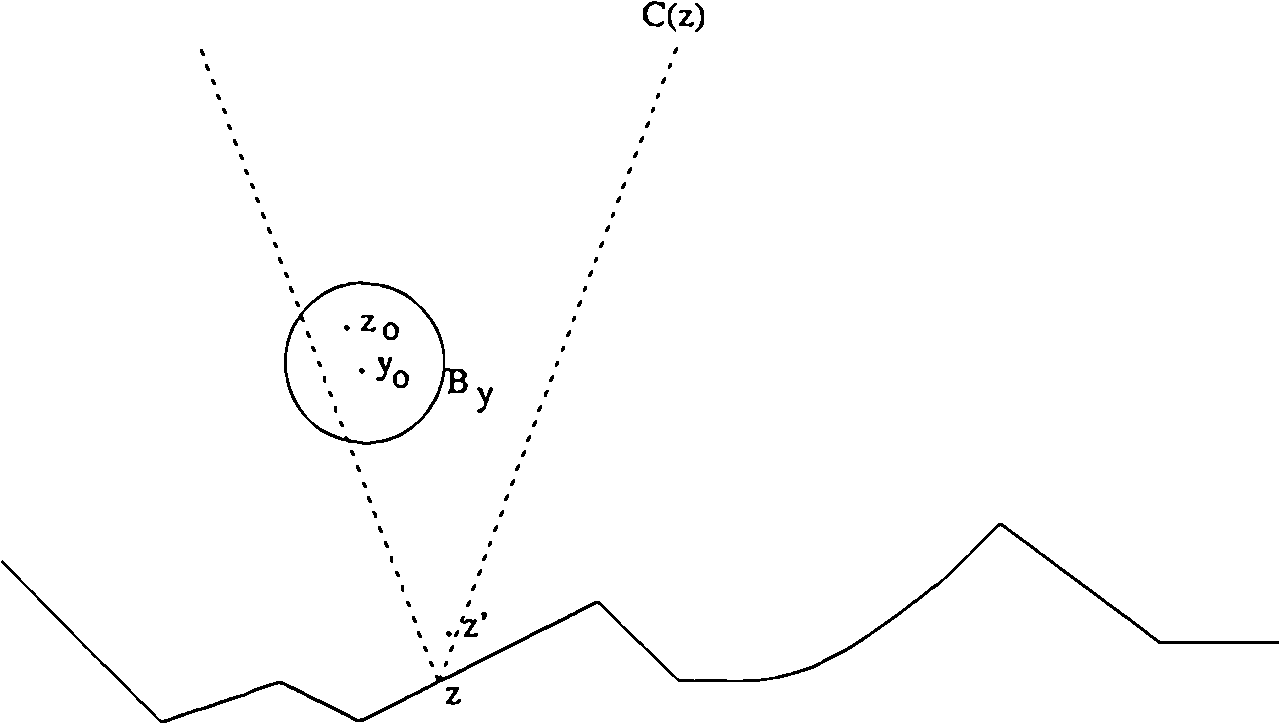
\includegraphics{Images/Img8.png}
    \bigskip
    \caption{Diagram for the proof of Proposition \ref{prop:ch3_4.2}.}
    \label{fig:ch3_4.1}
\end{figure}

\subsecbkm{ch3_sec4.2}{Fatou theorems}
\index{Fatou theorem|(}

Define $\omega^{x_0}(dz)$ by \eqref{eq:ch3_2.2}. We now can prove the following.

\begin{theorem}\label{thm:ch3_4.3}
Suppose $u$ is a nonnegative harmonic function in $D$. Then $\lim_{y \to z,y \in C(z)} u(y)$ exists for almost every $z \in \partial D$ with respect to $\omega^{x_0}(dz)$.
\end{theorem}

\begin{proof}
Let $U_t = u(X_{t \wedge \tau_D})$. For $t < \tau_D$, $U_t$ is a martingale that is bounded below by $0$, and by the martingale convergence theorem (Corollary \chapref[I]{eq:ch1_4.14}), $\lim_{t \to \tau_D} U_t$ exists, a.s.
\[
    1 = \P^{x_0}(\lim_{t \to \tau_D} U_t~\text{exists}) = \int \P_z^{x_0}(\lim_{t \to \tau_D} U_t~\text{exists})\omega^{x_0}(dz)
\]
by Proposition \ref{prop:ch3_2.7}. So for almost every $z$,
\[
    \P_z^{x_0}(\lim_{t \to \tau_D} U_t\text{~exists}) = 1.
\]
Let $N$ be the null set of $z$s for which the $\P_z^{x_0}$ probability is not 1 and fix a $z \not\in N$. We will show $\lim_{y \to z,y \in C(z)} u(y)$ exists for this $z$.

By the zero-one law Theorem \ref{thm:ch3_2.9}, there exists $L$ such that $U_t \to L$ as $t \to \tau_D$, $\P_z^{x_0}$-a.s.\ ($L$ depends on $z$.) If we have $\limsup_{y \to z,y \in C(z)} u(y) > L$, there exists $\epsilon$ and $y_1,y_2,\ldots \in C(z)$ such that $y_n \to z$ and $u(y_n) > L + \epsilon$. By Harnack's inequality, there exists $c_1$ small such that if $B_n = B(y_n,c_1\dist(y_n,\partial D))$, then $u \geq L + \epsilon/2$ on $B_n$. By Proposition \ref{prop:ch3_4.2}, there exists $c_2$ such that under $\P_z^{x_0}$, $X_t$ hits each $B_n$ with probability at least $c_2$. So if $A_n = (T_{B_n} < \tau_D)$, then
\begin{align*}
    \P_z^{x_0}(A_n~\text{i.o.}) &= \P_z^{x_0}(\cap_{j=1}^\infty \cup_{n=j}^\infty A_n) = \lim_{j \to \infty} \P_z^{x_0}(\cup_{n=j}^\infty A_n) \\
    &\geq \liminf_{j \to \infty} \P_z^{x_0}(A_j) \geq c_2.
\end{align*}
Therefore $\P_z^{x_0}(T_{B_n} < \tau_D~\text{i.o.}) > c_2$, and hence $\P_z^{x_0}(U_t > L + \epsilon/2~\text{i.o.}) > c_2$, contradicting $U_t \to L$. Thus $\limsup_{y \to z,y \in C(z)} u(y) \leq L$. Similarly, $\liminf_{y \to z,y \in C(z)} u(y) \geq L$, which proves the theorem.
\end{proof}

The following theorem is also known as a Fatou theorem.

\begin{theorem}\label{thm:ch3_4.4}
If $f \in L^p(\partial D,\omega^{x_0})$, $1 \leq p \leq \infty$, and $u(y) = \E^yf(X_{\tau_D})$, then
\[
    \lim_{y \to z,y \in C(z)} u(y) = f(z)
\]
for almost every $z \in \partial D$ with respect to $\omega^{x_0}$.
\end{theorem}

\begin{proof}
Writing $f = f^+ - f^-$, where $f^+,f^-$ are the positive and negative parts of $f$, respectively, it suffices to prove the theorem for $f \geq 0$. Now by the martingale convergence theorem, $U_t \to f(X_{\tau_D})$, a.s.\ as $t \to \tau_D$. So for almost every $z$, $U_t \to f(X_{\tau_D}) = f(z)$, $\P_z^{x_0}$-a.s. Now proceed as in the above proof with $L = f(z)$.
\end{proof}

\index{Fatou theorem|)}

\subsecbkm{ch3_sec4.3}{Maximal functions}
\index{Maximal function|(}

Closely related to the Fatou theorems are maximal function inequalities. Let $U_t = u(X_{t \wedge \tau_D})$, $U^* = \sup_{s < \tau_D} |U_s|$, and $N(f)(z) = \sup_{y \in C(z)} |u(y)|$.

\begin{theorem}\label{thm:ch3_4.5}
Suppose $f \in L^p(\partial D,\omega^{x_0})$ and let $u(y) = \E^yf(X_{\tau_D})$. Then there exists $c$ depending only on $p$ such that
\begin{equation}
    \omega^{x_0}(\{z: N(f)(z) > \lambda\}) \leq c\P^{x_0}(U^* > \lambda/4); \tag{a}
\end{equation}
\begin{equation}
    \int |N(f)(z)|^p\omega^{x_0}(dz) \leq c \int |f(z)|^p\omega^{x_0}(dz) \quad \text{if}~1 < p < \infty. \tag{b}
% Note: \quad is used here.
\end{equation}
\end{theorem}

We will still restrict ourselves to the case when $D$ is the region above
the graph of a bounded Lipschitz function. Exercise \ref{ex:ch3_17} asks the reader to
consider the case of bounded Lipschitz domains.

\begin{proof}
Since $f^+,f^- \leq |f|$ and $N(f)(z) \leq N(f^+)(z) + N(f^-)(z)$, we may again suppose $f \geq 0$. Let $A = \{z : N(f)(z) > \lambda\}$. If $z \in A$, there must exist $y \in C(z)$ with $u(y) > \lambda$. By Harnack's inequality, there exists $c_1$ independent of $y$ such that $u > \lambda/2$ on $B = B(y,c_1r)$, $r = \dist(y,\partial D)$. Then $\P_z^{x_0}(T_B < \tau_D) \geq c_2$, or $\P_z^{x_0}(U^* > \lambda/2) \geq c_2$. So by Proposition \ref{prop:ch3_2.7}
\begin{align}\label{eq:ch3_4.8}
    c_2\omega^{x_0}(A) &\leq \int_A \P_z^{x_0}(U^* > \lambda/2)\omega^{x_0}(dz) \\
    &= \int_A \P_z^{x_0}(U^* > \lambda/2)\P^{x_0}(X_{\tau_D} \in dz) \notag \\
    &= \P^{x_0}(U^* > \lambda/2, X_{\tau_D} \in A) \leq \P^{x_0}(U^* > \lambda/2), \notag
\end{align}
which is (a).

For (b), multiply (a) by $p\lambda^{p-1}$ and integrate over $\lambda$ from $0$ to $\infty$. Using Proposition \chapref[I]{prop:ch1_1.5} and Doob's inequality,
\begin{align*}
    \int |N(f)(z)|^p\omega^{x_0}(dz) &\leq c\E^x\big[(U^*)^p\big] \leq c\E^{x_0}\big[(f(X_{\tau_D}))^p\big] \\
    &= c \int f(z)^p\omega^{x_0}(dz).
\end{align*}
This gives (b).
\end{proof}

By taking $D$ equal to the ball, we can recover the usual maximal inequality and Fatou theorems (see Sect.\ \chapref[IV]{ch4_sec1}). For $D$ equal to the half-space, recall
\[
    \omega^{x_0}(dz) = \frac{cx_0^d}{(|x_0^d|^2 + |z_0 - z|^2)^{d/2}}dz,
\]
where $x_0^d$ is the $d$th coordinate of $x_0$. Multiplying by $(x_0^d)^{d-1}$ and letting $x_0^d \to \infty$, we obtain the corresponding theorems for the half-space. See Chap.\ \ref{ch4}, however, where things are done more directly.

\index{Maximal function|)}

\subsecbkm{ch3_sec4.4}{Extensions}

Note that the only ingredients needed in all of the above were scale invariance, the boundary Harnack principle, and Harnack's inequality. Suppose $D$ is a John domain\index{John domain} with \eqref{eq:ch3_1.31} holding, not only for $z \in D$, but for $z \in \partial D$. If $z \in \partial D$, let $\gamma_z$ be the arc connecting $x_0$ and $z$. For suitably small $b$, define
\[
    C(z) = \cup_{y \in \gamma_z} B(y,br_y),
\]
where $r_y = \ell(\gamma_z(y,z))$ and $\ell(\gamma_z(y,z))$ is the length of the piece of arc between $y$ and $z$. Then slight modifications of the above proofs show that the Fatou theorems hold for John domains.

\mnewpage

The usual analytic proofs of Fatou theorems proceed by first proving the maximal inequality Theorem \ref{thm:ch3_4.5}. One key step is to prove the doubling property of harmonic measure: there exists $c$ such that if $z \in \partial D$, then $\omega^{x_0}(B(z,2r)) \leq c\omega^{x_0}(B(z,r))$ for all $r$ (cf.\ Corollary \ref{cor:ch3_5.5}). One feature of the boundary Harnack principle proof is that it works for domains that might not have the doubling property (for example, it is not hard to find a John domain that does not have the doubling property: take a domain that has a sharp enough cusp pointing into it).

Can Fatou theorems be proved for more general domains than Lipschitz ones? If $D$ can be written as the union of countably many Lipschitz domains, the results can be derived for $D$ from the results above, but we have something else in mind. If $D$ is a simply connected domain in $\R^2$, then a conformal invariance argument shows that $\lim_{y \to z,y \in L_z} u(y)$ exists a.e.\ with respect to harmonic measure if $u$ is positive and harmonic in $D$ and $L_z$ is the flow line through $z$ determined by the vector field $\nabla g_D(x_0,\cdot)$. This means that if $y \in L_z$, then $L_z$ is parallel to $\nabla g_D(x_0,y)$, or alternatively, $L_z$ is the image under $\varphi$ of the radius connecting $\varphi^{-1}(z)$ to $0$, where $\varphi$ is the conformal map mapping the unit disk onto $D$ and taking the origin to $x_0$. The question is, can one make some sort of similar assertion for $d \geq 3$?

\section{Support of harmonic measure}\label{ch3_sec5}

\subsecbkm{ch3_sec5.1}{Smooth domains}

If one starts a Brownian motion at $x_0 \in D$, where $D$ is a Lipschitz domain, what can one say about the distribution of $X_{\tau_D}$? The sort of result one would like is that the $\P^{x_0}$ distribution of $X_{\tau_D}$ is mutually absolutely continuous with respect to surface measure on $\partial D$. Actually more can be said. In this section we establish the results obtained by \cite{Dahlberg1977} and reproved by different means in \cite{JerisonKenig1982a}\index{Dahlberg's theorem}. Our method is a blend of the two. We also give a probabilistic demonstration of Gehring's inequality, which is needed to obtain the sharpest results.

Let $\sigma$ denote surface measure on $\partial D$ and $\omega^{x_0}$ harmonic measure starting from $x_0$. That is, $\omega^{x_0}(A) = \P^{x_0}(X_{\tau_D} \in A)$, $A \subseteq \partial D$. The main result is the following.

\begin{theorem}\label{thm:ch3_5.1}
Let $D$ be either a bounded Lipschitz domain or else the region above the graph of a bounded Lipschitz function. Let $x_0 \in D$.
\begin{enumerate}
    \item $\omega$ is absolutely continuous with respect to $\sigma$;
    \item if $K$ is the Radon-Nikodym derivative of $\omega^{x_0}$ with respect to $\sigma$, there exists $\epsilon > 0$ such that $K$ is locally in $L^{2+\epsilon}(d\sigma)$;
    \item $\sigma$ is absolutely continuous with respect to $\omega^{x_0}$.
\end{enumerate}
\end{theorem}

\mpagebreak

The theorem says that harmonic measure and surface measure are mutually absolutely continuous, and the density is locally in $L^{2+\epsilon}$ with respect to surface measure. Easy examples (\cite[see][]{Dahlberg1977}) show that the $2+\epsilon$ cannot be improved upon in general. $K$ locally in $L^{2+\epsilon}(d\sigma)$ means that for each $M > 0$, $K1_{B(0,M)} \in L^{2+\epsilon}(d\sigma)$. For bounded domains, $K$ locally in $L^{2+\epsilon}(d\sigma)$ is precisely the same as $K \in L^{2+\epsilon}(d\sigma)$; we phrase the theorem this way to cover the case of regions above the graph of bounded Lipschitz functions as well.

Observe that Theorem \ref{thm:ch3_5.1} is essentially a local result. If Theorem \ref{thm:ch3_5.1} holds for regions $D$ above the graph of a Lipschitz function, we can obtain Theorem \ref{thm:ch3_5.1} easily for bounded domains. Let us therefore suppose we are in the situation that $D$ is the region above the graph of a Lipschitz function.

A set of the form $A = B(w,r) \cap \partial D$ for some $w \in \partial D$ will be called a surface ball.

Let $\partial u/\partial n = \nabla u \cdot n$ denote the normal derivative, where $n(x)$ is the unit vector normal to the boundary at $x$ pointing inwards. For Lipschitz domains, $n$ is only defined for a.e.\ $x$. (See Exercise \chapref[II.8]{ex:ch2_8}.)

Set $v = g_D(x_0,\cdot)$. Since $v = 0$ on $\partial D$, it is clear by the Lipschitz nature of $D$ that there exist two constants $c_1,c_2$ such that
\begin{equation}\label{eq:ch3_5.1}
    c_1\frac{\partial v}{\partial(x^d)} \leq \frac{\partial v}{\partial n} \leq c_2\frac{\partial v}{\partial(x^d)}.
\end{equation}

Let us suppose at first that $D$ is the region above the graph of a bounded $C^\infty$ function $\Gamma$. We will derive estimates on harmonic measure that do not depend on the smoothness of $\Gamma$ (beyond its Lipschitz constant), and we can then take a limit.

We begin by showing that for smooth domains, harmonic measure has a bounded density with respect to surface measure.

\begin{theorem}\label{thm:ch3_5.2}
Let $\Gamma$ be a $C^2$ function such that $\Gamma$ and its first and second derivatives are bounded. Suppose $D$ is the region above the graph of $\Gamma$, $x_0 \in D$. Then $\omega^{x_0}(dy) = \P^{x_0}(X_{\tau_D} \in dy)$ has a density with respect to surface measure on $\partial D$ that is bounded.
\end{theorem}

This theorem could be obtained as an easy consequence of some results from partial differential equations. We give a proof that uses only the tools we have already developed.

A domain $D$ satisfies a uniform exterior sphere condition if there exist $r > 0$ such that for all $z \in \partial D$, there exists a ball $B_z$ of radius $r$ contained in $D^c$ with $z \in B_z \cap \partial D$.

\tweakpage{0.5}

\begin{proof}
For simplicity we will assume $d \geq 3$. We start with an estimate on $g_D(x_0,y)$ for $y$ near the boundary of $D$. We show first that
\begin{obs}\label{obs:ch3_5.2}
    \textit{There exists $c$ and $a$ such that $g_D(x_0,y) \leq c\dist(y,\partial D)$ if $\dist(y,\partial D) \allowbreak \leq a$.}
\end{obs}

It is easy to see that the region above $\Gamma$ satisfies a uniform exterior sphere condition. Suppose $y \in D$. Let $z$ be a point of $\partial D$ that minimizes $|y - z|$ and let $B_z$ be a ball of radius $r$ contained in $D^c$ touching $\partial D$ at $z$. Then $g_D(x_0,y) \leq g_{B_z^c}(x_0,y)$ since $D \subseteq B_z^c$. \eqref{obs:ch3_5.2} follows by the explicit formula for $g_{B_z^c}$ (Proposition \chapref[II]{prop:ch2_3.9}).

Next is an estimate on $\nabla g_D(x_0,y)$. Suppose $y \in D$ and $r = \dist(y,\partial D) \allowbreak < a/2$. Since \eqref{obs:ch3_5.2} implies that $g_D(x_0,\cdot)$ is bounded by $2cr$ on $B(y,r)$, then from Corollary \chapref[II]{cor:ch2_1.4} we have
\begin{equation}\label{eq:ch3_5.3}
    |\nabla g_D(x_0,y)| \leq \frac{c}{r} \sup_{B(y,r)} |g_D(x_0,\cdot)| \leq c.
\end{equation}

Define $D_{+b}$ to be the region above $\Gamma(x^1,\ldots,x^{d-1}) + b$ and similarly $D_{-b}$. Let $f$ be a smooth nonnegative function with compact support defined on $\partial D$. Extend $f$ to all of $\R^d$ by defining $f(y) = f(w)$ if $w \in \partial D$ and $y$ is above or below $w$. Fix $b$ for the moment and let $v_b(x) = \E^xf(X_{\tau_{(D_{-b})}})$.

Let $M > 1$ and let us apply Green's second identity to the functions $v_b$ and $g_D$ in $D_{+\delta} \cap B(0,M) - B(x_0,\epsilon)$. Both $v_b$ and $g_D$ are harmonic and smooth in this region. We let $M \to \infty$ and argue that the terms involving $\partial B(0,M)$ go to $0$. $g_D(x_0,y) \leq u(x_0,y)$, the Newtonian potential, which is bounded by a constant if $y$ is within $(\delta \wedge \epsilon)/2$ of the boundary of $D \cap B(0,M) - B(x_0,\epsilon)$, and $g_D(x_0,y) \leq cM^{2-d}$ if $M$ is large enough and $y$ is within $(\delta \wedge \epsilon)/2$ of $D \cap \partial B(0,M)$. By Corollary \chapref[II]{cor:ch2_1.4}, $|\nabla g_D(x_0,y)|$ is bounded by $c(\delta,\epsilon)M^{2-d}$ for $y \in D_{+\delta} \cap \partial B(0,M)$. Since $f$ is bounded, $v_b$ is bounded, and again using Corollary \chapref[II]{cor:ch2_1.4}, $|\nabla v_b|$ is bounded on $D_{+\delta} \cap B(0,M)$. Since the surface area of $B(0,M)$ is less than $cM^{d-1}$, it follows that the terms involving the integral over $D_{+\delta} \cap B(0,M)$ tend to $0$ as $M \to \infty$.

We are thus left with
\[
    \int_{\partial D_{+\delta}} v_b\frac{\partial g_D}{\partial n} + \int_{\partial B(x_0,\epsilon)} v_b\frac{\partial g_D}{\partial n} = \int_{\partial D_{+\delta}} g_D\frac{\partial v_b}{\partial n} + \int_{\partial B(x_0,\epsilon)} g_D\frac{\partial v_b}{\partial n}.
\]
Precisely as in the proof of Proposition \chapref[II]{prop:ch2_3.11}, we can let $\epsilon \to 0$ and see that
\begin{equation}\label{eq:ch3_5.4}
    cv_b(x_0) + \int_{\partial D_{+\delta}} g_D\frac{\partial v_b}{\partial n} = \int_{\partial D_{+\delta}} v_b\frac{\partial g_D}{\partial n}
\end{equation}
(Recall that here $n$ denotes the inward normal while Green's identities are formulated in terms of the outward pointing normal.) Using \eqref{eq:ch3_5.3}, the right-hand side of \eqref{eq:ch3_5.4} is bounded by $c\int_{D_{+\delta}} v_b(y)\sigma(dy)$, which converges to $c\int_{\partial D} v_b(y)\sigma(dy)$ as $\delta \to 0$. By \eqref{obs:ch3_5.2} the left-hand side of \eqref{eq:ch3_5.4} converges to $cv_b(x_0)$.

\tweakpage{0.5}

Let $e_d$ be the unit vector in the $d$th coordinate direction. By translation invariance, $v_b(y) = v_0(y + be_d)$. Every point of $\partial D$ is regular for $D^c$; so if $y \in \partial D$, $v_b(y) = v_0(y + be_d) \to f(y)$ as $b \downarrow 0$. Also $v_b(x_0) = v_0(x_0 + be_d) \to v_0(x_0)$. Therefore we end up with
\mpagebreak
\begin{equation}\label{eq:ch3_5.5}
    \int_{\partial D} f(y)\omega^{x_0}(dy) = \E^{x_0}f(X_{\tau_D}) = v_0(x_0) = c\int_{\partial D} f(y)\sigma(dy).
\end{equation}
That $\omega^{x_0}$ has a bounded Radon-Nikodym derivative with respect to $\sigma$ follows immediately from \eqref{eq:ch3_5.5}.
\end{proof}

\subsecbkm{ch3_sec5.2}{\texorpdfstring{$L^2$}{L²} estimates}

We are now ready to show that $d\omega/d\sigma \in L^2(\sigma)$ for $C^\infty$ domains with estimates only depending on $M_\Gamma$ and not on any further smoothness. This will actually not take too long. The bulk of this section will be in deriving the $L^{2+\epsilon}$ estimate.

\begin{proposition}\label{prop:ch3_5.3}
Suppose $w \in \partial D$, $r > 0$, and $A = B(w,r) \cap \partial D$. Let $y_0$ be above $w$ with $\dist(y_0,\partial D) = r$. Then there exists $c$ such that
\begin{equation}\label{eq:ch3_5.6}
    \int_A \Big(\frac{d\omega^{y_0}}{d\sigma}(w)\Big)^2\sigma(dw) \leq c/\sigma(A).
\end{equation}
\end{proposition}

\begin{proof}
Pick $z_0$ above $w$ with $\dist(z_0,\partial D) = r/2$. By Harnack's inequality in $D$, there exists $c_1$ such that if $u$ is harmonic and positive in $D$, then $u(z_0)/u(y_0) \leq c_1$ and $u(y_0)/u(z_0) \leq c_1$. Take $\epsilon < 1/8$ small enough so that if $x \in B(z_0,\epsilon r)$, then $u(x)/u(z_0) \leq 2$. That this can be done follows by the expression for the constant in Harnack's inequality in Theorem II.1.19. Note if $x \in B(y_0,r/8)$, then $|x - z_0| \geq r/4$ and by Proposition \chapref[I]{prop:ch1_5.8}
\[
    \P^x(T_{B(z_0,\epsilon r)} < \infty) \leq \frac{(\epsilon r)^{d-2}}{(r/4)^{d-2}}.
\]
So take $\epsilon$ even smaller if necessary so that
\[
    \sup_{x\in B(y_0,r/8)} \P^x(T_{B(z_0,\epsilon r)} < \infty) \leq \frac{1}{4c_1}.
\]
Write $B$ for $B(z_0,\epsilon r)$.

Let $h(x) = g_D(x,z_0)$, $k(x) = (\partial h/\partial(x^d))(x)$, and for $x \in \partial D$, $L(x) = (\partial h/\partial n)(x)$. We want to show
\begin{equation}\label{eq:ch3_5.7}
    \int_A L^2(w)\sigma(dw) \leq c_3/\sigma(A).
\end{equation}

The key observation is that the left-hand side of \eqref{eq:ch3_5.7} is equal to $\int_A L(w)\omega^{z_0}(dw) = \E^{z_0}[L(X_{\tau_D}); X_{\tau_D} \in A]$. We use our choices of $\epsilon,z_0$, etc.\ to bound this in terms of $\E^{y_0}k(X_{\tau_D \wedge T_B})$.

Since $x \to \E^x(L1_A)(X_{\tau_D})$ is harmonic in $D$, then
\begin{equation}\label{eq:ch3_5.8}
    \E^{z_0}[L(X_{\tau_D}); X_{\tau_D} \in A] \leq c_1\E^{y_0}[L(X_{\tau_D}); X_{\tau_D} \in A].
\end{equation}
Now
\begin{align*}
    \E^{y_0}[L(X_{\tau_D})] &= \E^{y_0}[L(X_{\tau_D}); \tau_D < T_B] + \E^{y_0}[L(X_{\tau_D}); \tau_D > T_B] \\
    &= \E^{y_0}[L(X_{\tau_D}); \tau_D < T_B] + \E^{y_0}[\E^{X_{T_B}}L(X_{\tau_D}); \tau_D > T_B].
\end{align*}
Again, $\E^zL(X_{\tau_D})$ is a positive harmonic function. For $v \in B$,
\[
    \E^vL(X_{\tau_D}) \leq 2\E^{z_0}L(X_{\tau_D}) \leq 2c_1\E^{y_0}L(X_{\tau_D})
\]
by our choice of $\epsilon$. So
\begin{align*}
    \E^{y_0}L(X_{\tau_D}) &\leq \E^{y_0}[L(X_{\tau_D}); \tau_D < T_B] + 2c_1\E^{y_0}L(X_{\tau_D})\P^{y_0}(\tau_D > T_B) \\
    &\leq \E^{y_0}[L(X_{\tau_D}); \tau_D < T_B] + 2c_1\E^{y_0}L(X_{\tau_D})\P^{y_0}(T_B<\infty) \\
    &\leq \E^{y_0}[L(X_{\tau_D}); \tau_D < T_B] + \E^{y_0}L(X_{\tau_D})/2.
\end{align*}
Since our domain is smooth, $L$ is bounded. Hence
\begin{equation}\label{eq:ch3_5.9}
    \E^{y_0}[L(X_{\tau_D}); X_{\tau_D} \in A] \leq \E^{y_0}L(X_{\tau_D}) \leq \E^{y_0}[L(X_{\tau_D}); \tau_D < T_B].
\end{equation}
By \eqref{eq:ch3_5.1} this is less than or equal to
\begin{equation}\label{eq:ch3_5.10}
    2c\E^{y_0}[k(X_{\tau_D}); \tau_D < T_B] \leq 2c\E^{y_0}[k(X_{\tau_D \wedge T_B})].
\end{equation}
Note $k$ is harmonic on $D - B$. So $\E^{y_0}[k(X_{\tau_D \wedge T_B})] = k(y_0)$. Since
\[
    |\nabla h(y_0)| \leq cr^{-1} \sup_{B(y_0,r/8)} h,
\]
then
\begin{equation}\label{eq:ch3_5.11}
    k(y_0) \leq \frac{c}{r}r^{2-d} = cr^{1-d} \leq c/\sigma(A).
\end{equation}
Combining \eqref{eq:ch3_5.8}, \eqref{eq:ch3_5.9}, \eqref{eq:ch3_5.10}, and \eqref{eq:ch3_5.11}, we obtain \eqref{eq:ch3_5.7}, or
\begin{equation}\label{eq:ch3_5.12}
    \int_A \Big(\frac{d\omega^{z_0}}{d\sigma}(w)\Big)^2\sigma(dw) \leq c/\sigma(A).
\end{equation}
Finally, by Harnack's inequality (cf.\ the remarks following Definition \ref{def:ch3_2.5}), $\omega^{y_0}(B) \leq c\omega^{z_0}(B)$ for any Borel set $B$, so
\[
    d\omega^{y_0}/d\sigma \leq cd\omega^{z_0}/d\sigma.
\]
\end{proof}

A suitable approximation scheme gives us Theorem \ref{thm:ch3_5.1}(a). We approximate $D$ by smooth domains $D_n$. One way to construct the $D_n$s is as follows. Let $\varphi$ be a nonnegative $C^\infty$ function with compact support that is radially symmetric and has integral $1$. Let $\varphi_\epsilon(x) = \epsilon^{-d}\varphi(x/\epsilon)$. Let $\Gamma_n(x) = \varphi_{1/n} * \Gamma(x) - \alpha_n$, where $\alpha_n$ tends to $0$ slowly compared to $1/n$. Let $D_n$ be the region above $\Gamma_n$. Since $\alpha_n \to 0$, $D_n \to D$, and moreover the Lipschitz constants $M_{\Gamma_n}$ are uniformly bounded. Since $\alpha_n$ is chosen to tend to $0$ sufficiently slowly, $D \subseteq D_n$.

\begin{proof}[Proof of Theorem \ref{thm:ch3_5.1}(a)]
Let the $D_n$ be constructed as above. Fix $y_0$. Let $A$ be a surface ball in $\partial D$ and let $\widetilde{A}$ be the set of points in $D$ that are above points of $A$. Let $f$ be a nonnegative $C^\infty$ function with support in $A$ with $\int_{\partial D} f^2\sigma_D(dz) \leq 1$. Extend $f$ to $D$ by defining $f(y) = f(w)$ if $y$ is above $w \in A$. Let $\sigma_{D_n}$ be surface measure for the boundary of $D_n$ and let $L_n$ be the Radon-Nikodym derivative of $\P^{y_0}(X_{\tau(D_n)} \in \cdot)$ with respect to $\sigma_{D_n}$. Then
\begin{align*}
    \E^{y_0}f(X_{\tau_{D_n}}) &= \int_{\partial D_n} f(w)\P^{y_0}(X_{\tau_{D_n}} \in dw) = \int_{\partial D_n} f(w)L_n(w)\sigma_{D_n}(dw) \\
    &\leq \Big(\int_{\partial D_n} f^2(w)\sigma_{D_n}(dw)\Big)^{1/2}\Big(\int_{\partial D_n \cap \widetilde{A}} L_n^2(w)\sigma_{D_n}(dw)\Big)^{1/2} \\
    &\leq c\|f\|_{L^2(\sigma_{D_n})}/\sigma_{D_n}(\widetilde{A})^{1/2}.
\end{align*}
We used the Cauchy-Schwarz inequality in the second line.

It should be clear that $\|f\|_{L^2(\sigma_{D_n})} \leq c\|f\|_{L^2(\sigma)}$ and $\sigma_{D_n}(\widetilde{A}) \geq c\sigma(A)$. Since $X_t$ is continuous, $f$ is continuous, and $\tau_{D_n} \downarrow \tau_D$,
\[
    \int f(w)\omega^{y_0}(dw) = \E^{y_0}f(X_{\tau_D}) \leq c\|f\|_{L^2(\sigma)}/\sigma(A)^{1/2}.
\]

If $E \subseteq A$ is closed with $\sigma_D(E) = 0$, taking suitable $f$ decreasing to $1_E$ shows $\omega^{y_0}(E) = 0$. So $\omega^{y_0}$ restricted to $A$ is absolutely continuous with respect to $\sigma$ restricted to $A$. This proves (a), but let us obtain a further estimate. Let $L$ be the density of $\omega^{y_0}$ with respect to $\sigma$. Then
\[
    \int f(w)L(w)\sigma_D(dw) \leq c\|f\|_{L^2(\sigma)}/\sigma_D(A)^{1/2}.
\]
Taking the supremum over all such nonnegative $C^\infty$ functions $f$ with support in $A$ and with $\|f\|_{L^2(d\sigma)} \leq 1$ implies
\begin{equation}\label{eq:ch3_5.13}
    \Big(\int L^2(w)\sigma_D(dw)\Big)^{1/2} \leq c/\sigma_D(A)^{1/2}.
\end{equation}
\end{proof}

\subsecbkm{ch3_sec5.3}{Surface balls}

To prove Theorem \ref{thm:ch3_5.1}(b), the $L^{2+\epsilon}$ estimate, we need to work harder. First we need some estimates on the harmonic measure of surface balls\index{Surface balls}.

\begin{theorem}\label{thm:ch3_5.4}
Suppose $w \in \partial D$ and $A = B(w,r) \cap \partial D$. Let $y$ be above $w$ with $\dist(y,\partial D) = r$. Then there exist $c_1$ and $c_2$ such that
\mpagebreak
\[
    c_1g_D(x_0,y)r^{d-2} \leq \P^{x_0}(X_{\tau_D} \in A) \leq c_2g_D(x_0,y)r^{d-2}.
\]
\end{theorem}

\begin{proof}
Let $B = B(y,r/2)$. By the support theorem (Theorem \chapref[I]{thm:ch1_6.6}), if $z \in B$, $\P^z(X_{\tau_D} \in A) \geq c_3$. (We just draw a narrow tube centered about the line segment from $z$ to $w$.) Then by Proposition \ref{prop:ch3_4.1},
\begin{align*}
    \P^{x_0}(X_{\tau_D} \in A) &\geq \P^{x_0}(X_{\tau_D} \in A; T_B < \tau_D) \\
    &= \E^{x_0}\big[\P^{X_{T_B}}(X_{\tau_D} \in A); T_B < \tau_D\big] \\
    &\geq c\P^{x_0}(T_B < \tau_D) \geq cg_D(x_0,y)r^{d-2}.
\end{align*}

For the other direction, pick $z$ above $w$ with $\dist(z,\partial D) = 7r/8$. If $x \in A$, then by the boundary Harnack principle in $D - B(z,r/16)$,
\[
    M(z,x) \geq \frac{cg_D(z,y)}{g_D(x_0,y)}.
\]
Since $g_D(z,y) \geq g_{B(z,r/4)}(z,y) \geq cr^{2-d}$ by Proposition \chapref[II]{prop:ch2_3.9}, it follows that $M(z,x) \geq cr^{2-d}/g_D(x_0,y)$. Thus by Theorem \ref{thm:ch3_2.6},
\[
    1 \geq \P^z(X_{\tau_D} \in A) = \int_A M(z,x)\omega^{x_0}(dx) \geq c\frac{r^{2-d}}{g_D(x_0,y)}\omega^{x_0}(A),
\]
or $\omega^{x_0}(A) \leq cg_D(x_0,y)r^{d-2}$ as required.
\end{proof}

The following corollary, the doubling property\index{Doubling property} of harmonic measure, follows easily from Theorem \ref{thm:ch3_5.4} and Harnack's inequality.

\begin{corollary}\label{cor:ch3_5.5}
There exists $c$ such that for all $w \in \partial D$ and $r > 0$, $\omega^{x_0}(B(w,2r) \cap \partial D) \leq c\omega^{x_0}(B(w,r) \cap \partial D)$.
\end{corollary}

\begin{proposition}\label{prop:ch3_5.6}
Suppose $D$ is the region above the graph of a $C^\infty$ function. Let $w \in \partial D$, $r > 0$, $A = B(w,r) \cap \partial D$, and choose $y$ above $w$ with $\dist(y,\partial D) = r$. There exists $c$ such that if $E \subseteq A$, then
\[
    \P^{x_0}(X_{\tau_D} \in E) \leq c\P^{x_0}(X_{\tau_D} \in A)\P^y(X_{\tau_D} \in E).
\]
\end{proposition}

\begin{proof}
If we show $M(y,z)$ is bigger than $c/\P^{x_0}(X_{\tau_D} \in A)$ for $z \in A$, we will then have our result, since by Theorem \ref{thm:ch3_2.6},
\[
    \P^y(X_{\tau_D} \in E) = \int_E M(y,z)\omega^{x_0}(dz) \geq \frac{c}{\P^{x_0}(X_{\tau_D} \in A)}\omega^{x_0}(E).
\]
Pick $z_0$ above $w$ with $\dist(z_0,\partial D) = \dist(y,\partial D)/2$. By the boundary Harnack principle in $D - B(y,r/2)$, if $z \in A$, then
\[
    M(y,z) \geq cg_D(y,z_0)/g_D(x_0,z_0).
\]

As we have seen several times before,
\[
    g_D(y,z_0) \geq g_{B(y,r/2)}(y,z_0) \geq cr^{2-d}.
\]
By Harnack's inequality, $g_D(x_0,z_0) \leq cg_D(x_0,y)$. So
\[
    M(y,z) \geq cr^{2-d}/g_D(x_0,y).
\]
By Theorem \ref{thm:ch3_5.4}, this is larger than $c/\P^{x_0}(X_{\tau_D} \in A)$.
\end{proof}

If $K_y(z)$ is the density of $\omega^y$ with respect to $\sigma$, we have from Proposition \ref{prop:ch3_5.6} that
\begin{equation}\label{eq:ch3_5.14}
    cK_y(z) \geq K_{x_0}(z)/\omega^{x_0}(A).
\end{equation}

\begin{proposition}\label{prop:ch3_5.7}
Let $A$ be a surface ball. Then
\[
    \frac{1}{\sigma(A)} \int_A K_{x_0}^2(z)\sigma(dz) \leq c\Big[\frac{1}{\sigma(A)} \int_A K_{x_0}(z)\sigma(dz)\Big]^2.
\]
\end{proposition}

\begin{proof}
Let $y$ be above $w$ as before. By Proposition \ref{prop:ch3_5.3},
\begin{equation}\label{eq:ch3_5.15}
    \int_A K_y^2(z)\sigma(dz) \leq c/\sigma(A).
\end{equation}
As in the proof of Theorem \ref{thm:ch3_5.1}(a), we take a limit to see that \eqref{eq:ch3_5.15} is still valid in Lipschitz domains, not just $C^\infty$ domains. By \eqref{eq:ch3_5.14},
\[
    \frac{1}{[\omega^{x_0}(A)]^2} \int_A K_{x_0}^2(z)\sigma(dz) \leq c/\sigma(A),
\]
or
\[
    \frac{1}{\sigma(A)} \int_A K_{x_0}^2(z)\sigma(dz) \leq c\Big[\frac{\omega^{x_0}(A)}{\sigma(A)}\Big]^2.
\]
Since $\omega^{x_0}(A) = \int_A K_{x_0}(z)\sigma(dz)$, this gives what we wanted.
\end{proof}

\subsecbkm{ch3_sec5.4}{Reverse H\"older inequalities}

The inequality in Proposition \ref{prop:ch3_5.7} is known as a reverse H\"older inequality\index{Reverse H\"older inequality} because the converse inequality is an immediate consequence of H\"older's inequality. We now prove Gehring's inequality\index{Gehring's inequality|(}, which when combined with Proposition \ref{prop:ch3_5.7} will yield Theorem \ref{thm:ch3_5.1}(b). Our proof is the standard proof suitably modified into martingale terms. (See also \cite{DoleansDadeMeyer1979} for further results and references related to this topic.)

\begin{lemma}\label{lem:ch3_5.8}
Suppose $X$ is a nonnegative integrable martingale, $Y = X^p$ for some $p > 1$, and $Y$ is integrable. Let $X_n = \E[X\mid \FC_n]$, $Y_n = \E[Y\mid \FC_n]$. Suppose
\begin{enumerate}
    \item there exists $c_1$ such that $Y_n \leq c_1Y_{n-1}$, a.s., for all $n$;
    \item there exists $c_2$ such that $Y_n \leq c_2X_n^p$, a.s., for all $n$.
\end{enumerate}

Then there exists $c_3$ such that
\begin{equation}\label{eq:ch3_5.16}
    \E[X^p; X > \lambda] \leq c_3\lambda^{p-1}\E[X; X > \lambda].
\end{equation}
\end{lemma}

\begin{proof}
Without loss of generality we may assume $c_2 \geq 1$. Let $\beta = 2c_2^{1/p}\lambda$. Let $N = \inf\{n: Y_n \geq \beta^p\}$. Then
\begin{equation}\label{eq:ch3_5.17}
    Y_N \leq c_1Y_{N-1} \leq c_1\beta^p.
\end{equation}
Also, $\beta^p \leq Y_N \leq c_2X_N^p$, or
\begin{equation}\label{eq:ch3_5.18}
    X_N \geq c_2^{-1/p}\beta = 2\lambda.
\end{equation}
Let $c_4 = 2c_2^{1/p}$. If $X > c_4\lambda$, then $Y = X^p > c_4^p\lambda^p = \beta^p$. Since $Y_n \to Y$, a.s., then $Y_n > \beta^p$ for some $n$, or $N < \infty$ on the set where $X > c_4\lambda$.

We now bound $\E[X^p; X > c_4\lambda]$ in terms of $\P(N < \infty)$ and bound that in turn in terms of $\E[X; X > \lambda]$.
\begin{align}\label{eq:ch3_5.19}
    \E[X^p; X > c_4\lambda] &= \E[Y; X > c_4\lambda] \leq \E[Y; N < \infty] \\
    &= \E[Y_N; N < \infty] \leq c_1\beta^p\P(N < \infty) \notag
\end{align}
by \eqref{eq:ch3_5.17}. By \eqref{eq:ch3_5.18}
\begin{align}\label{eq:ch3_5.20}
    \P(N < \infty) &\leq \frac{\E[X_N; N < \infty]}{2\lambda} = \frac{\E[X; N < \infty]}{2\lambda} \\
    &\leq \frac{\E[X; N < \infty, X > \lambda]}{2\lambda} + \frac{\E[X; N < \infty, X \leq \lambda]}{2\lambda} \notag \\
    &\leq \frac{\E[X; X > \lambda]}{2\lambda} + \frac{\lambda\P(N < \infty)}{2\lambda}. \notag
\end{align}
So
\[
    \P(N < \infty) \leq 2\E[X; X > \lambda]/2\lambda = \E[X; X > \lambda]/\lambda.
\]
Combining \eqref{eq:ch3_5.19} and \eqref{eq:ch3_5.20},
\[
    \E[X^p; X > c_4\lambda] \leq c_5\lambda^{p-1}\E[X; X > \lambda].
\]

Observing that
\begin{align*}
    \E[X^p; X > \lambda] &= \E[X^p; X > c_4\lambda] + \E[X^p; c_4\lambda \geq X > \lambda] \\
    &\leq \E[X^p; X > c_4\lambda] + c_4^{p-1}\lambda^{p-1}\E[X; c_4\lambda \geq X > \lambda] \\
    &\leq (c_5 + c_4^{p-1})\lambda^{p-1}\E[X; X > \lambda]
\end{align*}
completes the proof.
\end{proof}

\index{Gehring's inequality|)}

\begin{theorem}[Gehring]\label{thm:ch3_5.9}
Let $X$ and $Y$ be as above. Then there exists $r > \allowbreak p$ and $c > 0$ such that $\E X^r \leq c\E X$.
\end{theorem}

$r$ and $c$ depend on $p$, $c_1$, and $c_2$.

\begin{proof}
Suppose first that $\E X^r < \infty$. We have
\begin{align*}
    \E[X^r; X > 1] &= \E[X^pX^{r-p}; X > 1] \\
    &= \E\Big[X^p\Big(1 + (r-p)\int_1^X \lambda^{r-p-1}d\lambda\Big); X > 1\Big] \\
    &= \E[X^p; X > 1] + (r-p)\int_1^\infty \lambda^{r-p-1}\E[X^p; X > \lambda]d\lambda \\
    &\leq \E[X^p; X > 1] + c(r-p)\int_1^\infty \lambda^{r-p-1}\lambda^{p-1}\E[X; X > \lambda]d\lambda
\end{align*}
by Lemma \ref{lem:ch3_5.8}. This in turn is equal to
\begin{align*}
    \E[X^p; X > 1] &+ c(r-p)\E\Big[X\int_1^X \lambda^{r-2}d\lambda; X > 1\Big] \\
    &\leq \E[X^p; X > 1] + \frac{c(r-p)}{r-1}\E[X^r; X > 1].
\end{align*}
If $r > p$ but $r-p$ is small enough so that $c(r-p)/(r-1) < 1/2$, then
\[
    \E[X^r; X > 1] \leq 2\E[X^p; X > 1] \leq c\E[X; X > 1].
\]
Finally
\begin{align*}
    \E X^r &= \E[X^r; X > 1] + \E[X^r; X \leq 1] \\
    &\leq c\E[X; X > 1] + \E[X; X \leq 1] \\
    &\leq (c + 1)\E X.
\end{align*}

To remove the restriction that $\E X^r < \infty$, let $X_N = X \wedge N$. By Exercise \ref{ex:ch3_19}, we have inequality \eqref{eq:ch3_5.16} with $c_3$ replaced by some $c_3'$ (independent of $N$). So $\E X_N^r \leq c\E X_N \leq c\E X$. Now let $N \to \infty$ and use Fatou's lemma.
\end{proof}

\subsecbkm{ch3_sec5.5}{\texorpdfstring{$L^{2+\epsilon}$}{L\string^\{2+ε\}} estimates}

We can now apply Gehring's inequality to prove part (b) of Theorem \ref{thm:ch3_5.1}.

\begin{proof}[Proof of Theorem \ref{thm:ch3_5.1}(b)]
Let $w \in \partial D$ and let $Q$ be a cube of side length $r$ centered at $w$. It suffices to show
\begin{equation}\label{eq:ch3_5.21}
    \int_{Q\cap\partial D} K^{2+\epsilon}(z)\sigma(dz) < \infty,
\end{equation}
where $K = K_{x_0} = d\omega^{x_0}/d\sigma$.

\mpagebreak

Define a probability measure $\P$ on $Q \cap \partial D$ by $\P(E) = \sigma(E \cap Q)/\sigma(Q \cap \partial D)$. We partition $Q$ into $2^{nd}$ equal subcubes, $R_i$, $i = 1,2,\ldots,2^{nd}$, and let $\FC_n$ be the $\sigma$-field generated by the sets $\partial D \cap R_i$, $i = 1,2,\ldots,2^{nd}$. Then if $X$ is a function on $Q$,
\[
    \E[X\mid \FC_n](x) = \frac{\int_R X(y)\sigma(dy)}{\sigma(R)}
\]
if $x \in R$ and $R$ is one of the $2^{nd}$ subcubes (cf.\ \chapeqref[I]{eq:ch1_4.2}).

If $B$ is the surface ball with the same center as $R$ and radius $\sqrt{d}R$, so that $B$ circumscribes $R$, then by Proposition \ref{prop:ch3_5.7},
\begin{align*}
    \frac{1}{\sigma(R)} \int_R K^2(y)\sigma(dy) &\leq c\int_B K^2(y)\sigma(dy)/\sigma(R) \\
    &\leq c\frac{\sigma(B)}{\sigma(R)}\Big(\frac{\omega^{x_0}(B)}{\sigma(B)}\Big)
\end{align*}
Since $\sigma(B)/\sigma(R)$ is bounded by a constant and $\omega^{x_0}(B) \leq c\omega^{x_0}(R)$ by the doubling property of harmonic measure, we have
\begin{equation}\label{eq:ch3_5.22}
    \frac{1}{\sigma(R)} \int_R K^2(y)\sigma(dy) \leq c\Big(\frac{\int_R K(y)\sigma(dy)}{\sigma(R)}\Big)^2.
\end{equation}

Now let $X(y) = K_{x_0}(y)$. We need to check the other hypotheses of Gehring's inequality. If $x \in R$, \eqref{eq:ch3_5.22} tells us that
\begin{align}\label{eq:ch3_5.23}
    \E[X^2\mid \FC_n](x) &= \frac{\int_R X^2(y)\sigma(dy)}{\sigma(R)} \\
    &\leq c\Big(\frac{\int_R X(y)\sigma(dy)}{\sigma(R)}\Big)^2 = c\big[\E[X\mid \FC_n](x)\big]^2. \notag
\end{align}
Also,
\begin{align*}
    \E[X^2\mid \FC_{n+1}](x) &= \frac{\int_{R'} X^2(y)\sigma(dy)}{\sigma(R')} \leq \frac{\sigma(R)}{\sigma(R')} \frac{\int_R X^2(y)\sigma(dy)}{\sigma(R)} \\
    &\leq c\E[X^2\mid \FC_n](x)
\end{align*}
if $x \in R' \subseteq R$, $R' \in \FC_{n+1}$, and $R \in \FC_n$. Then by Gehring's inequality, $\E X^{2+\epsilon} < \infty$ for some $\epsilon > 0$. That is \eqref{eq:ch3_5.21} and we are done.
\end{proof}

Gehring's inequality is closely tied with the theory of $A_p$ weights\index{AA3@$A_p$ weights|(}. Let $\nu$ be a measure on a cube $Q_0$ with the doubling property. A positive function $w$ satisfies the $A_p$ condition for some $p \in (1,\infty)$ if
\[
    \sup \Big(\frac{1}{\nu(Q)} \int_Q w\,d\nu\Big)\Big(\frac{1}{\nu(Q)} \int_Q \Big(\frac{1}{w}\Big)^{1/(p-1)}d\nu\Big)^{p-1} < \infty,
\]
where the supremum is over all subcubes $Q$ of $Q_0$.

\mpagebreak

The relevance to us is the following.

\begin{theorem}\label{thm:ch3_5.10}
$K(z)$ is an $A_2$ weight with respect to $\omega^{x_0}(dz)$.
\end{theorem}

\begin{proof}
Let $\nu = \omega^{x_0}$. We have
\[
    \frac{1}{\sigma(R)} \int_R K^2(z)\sigma(dz) \leq c\Big(\frac{1}{\sigma(R)} \int_R K(z)\sigma(dz)\Big)^2.
\]
Let $w(x) = K(x)$. Then we write
\[
    \sigma(R) \int_R K(z)\nu(dz) \leq c\Big(\int \nu(dz)\Big)^2,
\]
or
\[
    \Big(\frac{1}{\nu(R)} \int_R \frac{1}{K(z)}\nu(dz)\Big)\Big(\frac{1}{\nu(R)} \int_R K(z)\nu(dz)\Big) \leq c.
\]
Thus $w$ is an $A_2$ weight with respect to $\nu$.
\end{proof}

See Exercise \ref{ex:ch3_20}, \cite{Garnett1981}, or \cite{CoifmanFefferman1974} for more on $A_p$ weights\index{AA3@$A_p$ weights|)}.

\subsecbkm{ch3_sec5.6}{Mutual absolute continuity}

We now prove Theorem \ref{thm:ch3_5.1}(c). Define $\mu$ on $\partial D$ by
\begin{equation}\label{eq:ch3_5.24}
    \mu(E) = \big|\big\{(x^1,\ldots,x^{d-1}) : (x^1,\ldots,x^{d-1},\Gamma(x^1,\ldots,x^{d-1})) \in E\big\}\big|.
\end{equation}
Note there exist $c_1$ and $c_2$ such that $c_1 \leq d\mu/d\sigma \leq c_2$.

\begin{proof}[Proof of Theorem \ref{thm:ch3_5.1}(c)]
Suppose $\sigma(E) > 0$ but $\omega^{y_0}(E) = 0$. Let $Q_{zk}$ denote the cube of the form $[j_1/2^k,(j_1+1)/2^k] \times \cdots \times [j_d/2^k,(j_d+1)/2^k]$ which contains $z$, where $j_1,\ldots,j_d$ are integers. By Exercise \ref{ex:ch3_13}, there exists $z \in E$ such that
\begin{equation}\label{eq:ch3_5.25}
    \frac{\mu(Q_{zk} \cap E)}{\mu(Q_{zk})} \to 1.
\end{equation}
(In fact, this is true for almost every point of $E$.)

Let
\[
    I_k = Q_{zk} \cap \partial D \qquad\text{and}\qquad E_k = I_k \cap E.
\]
Let $z_k$ be a point above $z$ with $\delta(z_k) = 2^{-k}$. [Recall the definition of $\delta(x)$ from \eqref{eq:ch3_1.6}.]

By scaling and the support theorem (Theorem \chapref[I]{thm:ch1_6.6}), $\omega^{z_k}(I_k) = \P^{z_k}(X_{\tau_D} \in I_k) \geq c$ (cf.\ the proof of Theorem \ref{thm:ch3_5.4}). Since $\omega^{y_0}(E) = 0$, then $\omega^{z_k}(E) = 0$ by Harnack's inequality. If $w_k$ is the center of $Q_{2k}$, let $\widehat{w}_k$ be the point above $w_k$ with $\delta(\widehat{w}_k) = 2^{-k}$. Then by Harnack's inequality again, there exists $c$ such that $d\omega^{z_k}/d\omega^{\widehat{w}_k} \leq c$. Hence $d\omega^{z_k}/d\sigma$ has a density $H_k$ in $L^2(\sigma)$ with $\int_{I_k} H_k^2(w)\sigma(dw) \leq c/\sigma(I_k)$.

\mpagebreak

So
\begin{align*}
    \omega^{z_k}(I_k - E_k) &= \int_{I_k-E_k} H_k(w)\sigma(dw) \\
    &\leq c\Big(\sigma(I_k)^{-1}\Big)^{1/2}\Big(\sigma(I_k - E_k)\Big)^{1/2}
\end{align*}
by the Cauchy-Schwarz inequality. This is less than or equal to
\[
    c\Big[\frac{\mu(I_k - E_k)}{\mu(I_k)}\Big]^{1/2} = c\Big[1 - \frac{\mu(I_k \cap E_k)}{\mu(I_k)}\Big]^{1/2} \to 0.
\]
This is a contradiction to $\omega^{z_k}(E_k) = 0$.
\end{proof}

We could actually have done this proof immediately following the proof of Theorem \ref{thm:ch3_5.1}(a), except for the minor details of switching from balls to cubes. If we had looked ahead and used Theorem \chapref[IV]{thm:ch4_1.2} and let $Q_{z_k}$ be the ball about $z$ of radius $2^{-n}$, we could have avoided using cubes altogether.

\subsecbkm{ch3_sec5.7}{Extensions}

A Lipschitz function is one where $\nabla\Gamma \in L^\infty$. We can define $L_1^p$ domains to be ones that are given locally as the region above the graph of a function $\Gamma$ with $\nabla\Gamma \in L^p$. \cite{JerisonKenig1981} have obtained the analog of Theorem \ref{thm:ch3_5.1} for $L_1^p$ domains when $p > d - 1$.

Some of the results concerning the Dirichlet problem in Lipschitz domains can also be approached via layer potentials\index{Layer potentials}. See \cite{Verchota1984}, \cite{FabesJodeitRiviere1978}, and \cite{JerisonKenig1982a}.

Suppose one considers regions above the graph of a function that is not necessarily Lipschitz. What can one say about the support of harmonic measure? It is not true in general that $\omega^{x_0} \ll \mu$, where $\mu$ is defined by \eqref{eq:ch3_5.24}. One can even find domains with finite surface measure for which this is not true. One might assert that harmonic measure is supported on those points where $\Gamma$ is differentiable. This also is not precisely true because one can perturb the domain by sets of small capacity without affecting things too much. Can one give a more exact condition?

\section{Exercises and further results}\label{ch3_sec6}

\begin{exercise}\label{ex:ch3_1}
Suppose $\Gamma$ is a continuous (not necessarily Lipschitz) bounded function and $D$ is the region above the graph of $\Gamma$. Suppose every point of $\partial D$ is regular for $D^c$. Suppose $x_1 \in \partial D$ and $x_0 \in D$ with $\delta(x_0) = 1$. Suppose that the conclusion of Theorem \ref{thm:ch3_1.2} holds with $K = \overline{B(x_1,2)}$ and $V = B(x_0,4)$. Show there exists $c$ such that if $u$ is positive and harmonic in $D$, $u$ vanishes continuously on $B(x_0,4) \cap \partial D$, and $u(x_0) = 1$, then $u$ is bounded by $c$ on $B(x_0,2) \cap D$. In other words, the boundary Harnack principle implies Carleson's estimate.
\end{exercise}

\begin{exercise}\label{ex:ch3_2}
Let $D$ be the region above the graph of a continuous (not necessarily Lipschitz) region and let $F_a = \{x \in D : \delta(x) < a\}$. Show there exists $\rho < 1$ such that $|\partial B(z,2a) \cap F_a| \leq \rho|\partial B(z,2a)|$ whenever $z \in F_a$.
\end{exercise}

\begin{exercise}\label{ex:ch3_3}
Suppose $D$ is the region above the graph of a H\"older function [see \eqref{eq:ch3_1.32}]. State and prove the appropriate analog to Lemma \ref{lem:ch3_1.6}.
\end{exercise}

\begin{exercise}\label{ex:ch3_4}
Prove \eqref{eq:ch3_1.20} and \eqref{eq:ch3_1.21}.
\end{exercise}

\begin{exercise}\label{ex:ch3_5}
Let $D_1$ and $D_2$ be two Lipschitz domains and let $r > 0$ so that $B(0,r) \cap D_1 = B(0,r) \cap D_2 \neq \emptyset$. Suppose $g_{D_1}$ has a finite strictly positive normal derivative on $B(0,r/2) \cap \partial D$. Prove that $g_{D_2}$ has a finite strictly positive normal derivative on $B(0,r/2) \cap \partial D$.
\end{exercise}

\begin{exercise}\label{ex:ch3_6}
Suppose $K$ is a compact set contained in an open set $V$ and there exists $c$ such that $g_D(x,y)/g_D(x',y) \leq c$ whenever $x,x' \in K \cap D$, $y \in D \cap \partial V$. Show the boundary Harnack inequality holds for the triple $(K,V,D)$.
\end{exercise}

\begin{exercise}\label{ex:ch3_7}
Let $\{G_i\}$ be a finite collection of bounded open sets covering a compact set $F \subseteq \R^d$. A $C^\infty$ partition of unity\index{Partition of unity} subordinate to $\{G_i\}$ is a collection of $C_F^\infty$ functions $h_i$ such that the support of $h_i$ is contained in $G_i$ for each $i$ and $\sum_i h_i = 1$ on $F$. Prove a partition of unity exists.
\end{exercise}

\begin{exercise}\label{ex:ch3_8}
Suppose $D$ is a bounded Lipschitz domain, $f$ is a function defined on $\partial D$, and for each $x \in \partial D$, there exists a $C^\infty$ function $h_x : \R^d \to \R$ and $r_x > 0$ such that $f$ agrees with $h_x$ in $B(x,r_x)$. Show there exists a $C^\infty$ function $h : \R^d \to \R$ such that $f$ is the restriction of $h$ to $\partial D$.

\hint Use a partition of unity.
\end{exercise}

\begin{exercise}\label{ex:ch3_9}
Let $D$ be a Lipschitz domain. Show there exists a constant $c$ depending only on $D$ such that if $y \in D$, then we have the boundary Harnack principle in $D - B(y,r)$ (i.e., the conclusion of Theorem \ref{thm:ch3_1.2} holds) with constant $c$ provided $r < \dist(y,\partial D)$.
\end{exercise}

\begin{exercise}\label{ex:ch3_10}
Suppose $D$ is a Lipschitz domain, $u$ and $v$ are positive and continuous, and $u$ and $v$ vanish continuously on $V \cap \partial D$ for some open set $V$. Show $u/v$ is H\"older continuous on $K \cap D$ if $K$ is a compact subset of $V$.
\end{exercise}

\begin{exercise}\label{ex:ch3_11}
Let $\Gamma$ be a Lipschitz function and $D$ the region above the graph of $\Gamma$. Show there exists a constant $c$ such that for all $r$ and $x$, we have the boundary Harnack principle in $Q(x,r,r)$ (i.e., the conclusion of Theorem \ref{thm:ch3_1.2} holds) with constant $c$.
\end{exercise}

\begin{exercise}\label{ex:ch3_12}
Suppose $f$ is a bounded function and there exists $\rho < 1$ such that $\Osc_{B(x,r)} f \leq \rho\Osc_{B(x,2r)} f$ for all $x$ and all $r < 1$. Show $f$ is H\"older continuous.

\mpagebreak

\hint The hypothesis implies that if $y \in B(x,2^{-n})$, then $|f(x)-f(y)| \leq \rho^n\|f\|_\infty$.
\end{exercise}

\begin{exercise}\label{ex:ch3_13}
\begin{enumerate}[wide, labelindent=0em, labelwidth=\parindent, labelsep = 0em]
    \item Let $\FC_n$ be an increasing collection of $\sigma$-fields on $\R^d$ such that each $\FC_n$ is generated by finitely many disjoint sets $A_{n1},\ldots,A_{nm_n}$. Show that if $\nu$ is a finite measure, $f \geq 0$ is integrable, and
    \[
        g_n(x) = \sum_{i=1}^{m_n} \frac{\int_{A_{ni}} f\,d\nu}{\nu(A_{ni})}1_{A_{ni}}(x),
    \]
    (with the convention $0/0 = 0$), then $g_n(x) \to f(x)$ for almost every $x$.
    \item Use (a) to prove \eqref{eq:ch3_2.3}.
    \item Use (a) to prove \eqref{eq:ch3_5.25}.
\end{enumerate}

\hint Cf.\ Exercise \chapref[I.8]{ex:ch1_16}.
\end{exercise}

\begin{exercise}\label{ex:ch3_14}
Suppose $D$ is a Lipschitz domain, $z \in \partial D$, and $(\P_z^x,X_t)$ is Brownian motion $h$-path transformed by the harmonic function $M(\cdot,z)$. If $x_0 \in \partial D$, show $\P_z^x$ has a weak limit as $x \to x_0$ with $x \in D$. We call the weak limit $\P_{z}^{x_0}$.

\hint Use the boundary Harnack principle to show tightness. Use the arguments of Sect.\ \ref{ch3_sec2} to show the limit exists.
\end{exercise}

\begin{exercise}\label{ex:ch3_15}
Show that $q$ is in the Kato class if and only if
\[
    \limsup_{K \to \infty} \sup_{x \in D} \int \frac{|q(y)|1_{(|q(y)| \geq K)}}{|x-y|^{d-2}}dy = 0.
\]
\end{exercise}

\begin{exercise}\label{ex:ch3_16}
If $q \geq 0$ and $\sup_{x \in D} \E^x \int_0^{\tau_D} q(X_s)ds < \infty$, show
\[
    \sup_{x \in \overline{D}} \E_z^x \int_0^{\tau_D} q(X_s)ds < \infty.
\]
\end{exercise}

\begin{exercise}\label{ex:ch3_17}
State and prove the analog of Theorem \ref{thm:ch3_4.5} for bounded Lipschitz domains.

\hint The definition of $C(z)$ needs to be modified.
\end{exercise}

\begin{exercise}\label{ex:ch3_18}
Suppose $f$ is a nonnegative function, $p > 1$, $c > 1$, and
\[
    \frac{1}{|Q|} \int_Q f(x)^p dx \leq \Big(\frac{c}{|Q|} \int_Q f(x)dx\Big)^p
\]
for all cubes $Q$. Show $f > 0$, a.e.
\end{exercise}

\begin{exercise}\label{ex:ch3_19}
Suppose $X \geq 0$, $p > 1$, and there exists $c_1$ such that for all $\lambda$,
\[
    \E[X^p; X > \lambda] \leq c_1\lambda^{p-1}\E[X; X > \lambda].
\]
Let $X_N = X \wedge N$. Show there exists $c_2$, independent of $N$ and $X$, such that
\mpagebreak
\[
    \E[X_N^p; X_N > \lambda] \leq c_2\lambda^{p-1}\E[X_N; X_N > \lambda].
\]

\hint Choose $c_3$ large but fixed. For $\lambda$ such that $N < \lambda$ or $\lambda \leq N < c_3\lambda$, the result is easy. For $\lambda \leq c_3^{-1}N$, use the inequality
\begin{align*}
    \E[X^p - N^p; X > N] &\geq pN^{p-1}\E[X - N; X > N] \\
    &\geq pc_3^{p-1}\lambda^{p-1}\E[X - N; X > N].
\end{align*}
\end{exercise}

\begin{exercise}\label{ex:ch3_20}
Suppose $w$ is an $A_p$ weight\index{AA3@$A_p$ weights}. (a) Show that $w$ is an $A_r$ weight for all $r > p$. (b) Show there exists $\epsilon > 0$ such that $w$ is an $A_{p-\epsilon}$ weight.

\hint Use Gehring's inequality.
\end{exercise}

\begin{exercise}\label{ex:ch3_21}
Let $D$ be a region as in Theorem \ref{thm:ch3_5.2}. (a) Show that $D$ satisfies a uniform interior sphere condition (i.e., the uniform exterior sphere condition for $D^c$). (b) Use (a) to prove there exists $c > 0$ such that $d\omega^{x_0}/d\sigma \geq c$.
\end{exercise}

\begin{exercise}\label{ex:ch3_22}
For each $\epsilon > 0$ construct an example where $d\omega^{x_0}/d\sigma$ is not locally in $L^{2+\epsilon}(d\sigma)$.

\hint Look at $d = 2$ and look at a wedge with the appropriate aperture.
\end{exercise}

\begin{exercise}\label{ex:ch3_23}
Give an example of a John domain\index{John domain} where harmonic measure does not have the doubling property\index{Doubling property}.

\hint Let $d = 2$ and let $D$ be the unit ball with the interval $[0,1] \times \{0\}$ removed.
\end{exercise}

\begin{exercise}\label{ex:ch3_24}
Show that harmonic functions are real analytic\index{Real analytic}. That is, if $x$ is in a domain $D$ and $h$ is harmonic in $D$, then $h$ can be expanded in a Taylor series about $x$ with radius of convergence equal to $\dist(x,\partial D)$.

\hint Show it first for the Poisson kernel in a ball.
\end{exercise}

\begin{exercise}\label{ex:ch3_25}
Suppose $h$ is a nonconstant harmonic function in a domain $D$. Show there cannot exist a subdomain on which $h$ is constant.

\hint Use Exercise \ref{ex:ch3_24}.
\end{exercise}

\begin{exercise}\label{ex:ch3_26}
Let $p$, $Y_i$, and $Z_n$ be as in Proposition \ref{prop:ch3_3.1}. Show
\[
    \P^1(Z_k~\text{ever hits}~0) < 1.
\]

\hint Cf.\ Exercise \chapref[I.8]{ex:ch1_18}.
\end{exercise}

\notessection
\addcontentsline{toc}{section}{Notes}

The boundary Harnack principle for Lipschitz domains was proved by \cite{Dahlberg1977}, \cite{Ancona1978}, and \cite{Wu1978}. Later, another proof was given by \cite{JerisonKenig1982a} and still another, a probabilistic one, was given in \cite{BassBurdzy1990}. A proof can be given using heat kernel estimates (\cite{Banuelos1992}). The proof using the box method follows \cite{BassBurdzy1990}. The proof using the SDE method is new.

The results on the Martin boundary were first established by \cite{HuntWheeden1970} in 1970, well before the boundary Harnack principle. Other proofs have been given by \cite{JerisonKenig1982a} and \cite{BassBurdzy1990}. We follow the proof of \cite{BassBurdzy1990}.

The conditional lifetime problem was posed by K.L. Chung around 1983 and solved in domains in $\R^2$ shortly thereafter by \cite{CranstonMcConnell1983}. For Lipschitz domains in $\R^d$ the results were first obtained in \cite{Cranston1985}. The proof given here follows \cite{BassBurdzy1992}; see that paper for many other references to the literature. Our account of the conditional gauge material and the three G theorem follows \cite{CranstonFabesZhao1988}.

The original Fatou theorems are classical. See, for example, \cite{Doob1984}. Some of our approach comes from \cite{Durrett1984}. The Fatou theorem for Lipschitz domains was first proved by \cite{HuntWheeden1968}. The idea of proving a Fatou theorem using the boundary Harnack principle has its roots in \cite{Doob1984}.

Theorem \ref{thm:ch3_5.1} was first proved by \cite{Dahlberg1977}, with a later proof by \cite{JerisonKenig1982a}.